%!TeX TS-program = Lualatex
%!TeX encoding = UTF-8 Unicode
%!TeX spellcheck = fr-FR
%!BIB TS-program = biber
% -*- coding: UTF-8; -*-
% vim: set fenc=utf-8
% based on 2017_backup/archives/2017_science/2017_CNRS/2017-02-01_évaluation/
\documentclass[11pt,french,a4paper,oneside]{article}%,twoside,draft
%============ common ===================
\usepackage[utf8]{inputenc}%
\usepackage[french]{babel}%
\usepackage{csquotes}%
\usepackage{etaremune}%
\usepackage[final]{pdfpages}%
%% --- unit formatting ---
\usepackage{microtype}	% Better typography \tolerance 1414
\hbadness 1414
\emergencystretch 1.5em
\hfuzz 0.3pt
\widowpenalty=10000
\vfuzz \hfuzz
\raggedbottom
%%%%%%%%%%%%%%%%%%%%%%%%%%%%%%%%%%%%%%%%%%%%%%%%%%%%%%%%%%%%%%%%%%%%%
\usepackage{amsmath,amsfonts,amsthm}			% Math packages
\usepackage{bm}%This package defines commands to access bold math symbols
\usepackage{graphicx}					% Enable pdflatex
%============ front-matter ===================
\newcommand{\BookTitle}{Centre National de la Recherche Scientifique}
\newcommand{\Title}{%
Rapport d'activité scientifique sur les travaux effectués
}%
\newcommand{\SubTitle}{%
Pour évaluation par les sections du Comité national}%
\newcommand{\Author}{Laurent U.~Perrinet}%
\newcommand{\Team}{\'Equipe NEural OPerations in TOpographies (NeOpTo)}%
\newcommand{\Institute}{Institut de Neurosciences de la Timone}%
\newcommand{\InstituteUMR}{UMR 7289, CNRS / Aix-Marseille Université}%
\newcommand{\Address}{27, Bd. Jean Moulin, 13385 Marseille Cedex 5, France}
\newcommand{\Website}{https://laurentperrinet.github.io/}
\newcommand{\Email}{Laurent.Perrinet@univ-amu.fr}
%%%%%%%%%%%%%%%%%%
%BIBLIOGRAPHY
%%%%%%%%%%%%%%%%%%
\usepackage[natbib=true,
			bibencoding=utf8,
%			encoding=utf8,
			maxcitenames=7,
			maxnames=7,
			%minnames=3,
			maxbibnames=7,
            sortcites=true,
            block=space,
            backend=biber,
%            doi=false,isbn=false,url=false,
            citestyle=alphabetic,%authoryear-comp,
            backref=true,
%            bibstyle=alphabetic
            ]{biblatex}%
\addbibresource{../2020-07-06_Perrinet20PredictiveProcessing/Perrinet20PredictiveProcessing.bib}
\addbibresource{~/github/perrinet_curriculum-vitae_tex/LaurentPerrinet_Publications.bib}
\addbibresource{~/github/perrinet_curriculum-vitae_tex/LaurentPerrinet_Presentations.bib}
\addbibresource{babel.bib}
%\usepackage[normalem]{ulem} %for \uline{}
%\DeclareNameFormat{given-family}{
%  \ifgiveninits
%  {\ifthenelse{\equal{\namepartfamily}{Toto}}
%    {\uline{\namepartfamily\addspace\namepartgiveni\namepartsuffix}}
%    {\namepartfamily\addspace\namepartgiveni\namepartsuffix}
%    \ifthenelse{\value{listcount} < \value{liststop}}
%    {\addcomma}
%    {\ifthenelse{\ifmorenames}{~et \,al \adddot}}
%    {}
%  }
%}
% https://tex.stackexchange.com/questions/359311/how-to-underline-name-of-specific-authors-in-biblatex
\usepackage{xpatch}
\usepackage[normalem]{ulem}

\newbox\savenamebox

%\newbibmacro*{name:bbold}[2]{%
%  \def\do##1{\iffieldequalstr{hash}{##1}{\bfseries\setbox\savenamebox\hbox\bgroup \listbreak}{}}%
%  \dolistloop{\boldnames}%
%}
\newbibmacro*{name:bbold}[2]{%
  \def\do##1{\iffieldequalstr{hash}{##1}{\setbox\savenamebox\hbox\bgroup \listbreak}{}}%
  \dolistloop{\boldnames}%
}

\newbibmacro*{name:ebold}[2]{%
  \def\do##1{\iffieldequalstr{hash}{##1}{\egroup\uline{\usebox\savenamebox}\listbreak}{}}%
  \dolistloop{\boldnames}%
}

\xpatchbibmacro{name:given-family}{\usebibmacro{name:delim}{#2#3#1}}{\usebibmacro{name:delim}{#2#3#1}\begingroup\usebibmacro{name:bbold}{#1}{#2}}{}{}

%\xpretobibmacro{name:given-family}{\begingroup\usebibmacro{name:bbold}{#1}{#2}}{}{}
\xapptobibmacro{name:delim}{\begingroup\normalfont}{}{}

\xapptobibmacro{name:given-family}{\usebibmacro{name:ebold}{#1}{#2}\endgroup}{}{}
\xapptobibmacro{name:delim}{\endgroup}{}{}

\newcommand*{\boldnames}{}
\forcsvlist{\listadd\boldnames}{
  {8fa031352aa34db95f5c1022358042a3}, % InBold
  {01b588ba4e4ad753feae6c81709fc04b}} % Highlight

%%%%%%%%%%%%%%%%%%%%%%%%%%%%%%
%% OPTIONAL MACRO FILES
%\usepackage{fltpage}
%\usepackage{tikz}
%%%%%%%%%%%%%%%%%%
%\usepackage{multicol}
%\usepackage{nag}
%============ graphics ===================
\usepackage{graphicx}
%============ hyperref ===================
\usepackage[unicode,linkcolor=blue,citecolor=blue,filecolor=black,urlcolor=blue,%pdfborder={0 0 0}
]{hyperref}%
\hypersetup{%
unicode = true, %
pdftitle={\Title},%
pdfauthor={\Author < \Email > - \Institute, \InstituteUMR , \Address - \Website},%
pdfsubject={\Title}%
}%
%\hypersetup{linkcolor=blue,citecolor=blue,filecolor=black,urlcolor=blue}
%\hyphenpenalty=5000
%\tolerance=1000
%% DOCUMENT LAYOUT
%\usepackage{geometry}
%\geometry{a4paper, textwidth=5.5in, textheight=8.5in, marginparsep=7pt, marginparwidth=.6in}
%\setlength\parindent{0in}
%% ---- MARGIN YEARS
\newcommand{\years}[1]{\marginpar{\textit{\scriptsize #1}}}
\providecommand{\natexlab}[1]{#1}
%\providecommand{\url}[1]{\texttt{#1}}
%\expandafter\ifx\csname urlstyle\endcsname\relax
 \providecommand{\doi}[1]{doi: #1}%\else
%  \providecommand{\doi}{doi: \begingroup \urlstyle{rm}\Url}\fi
%\makepagestyle{chapter}
%\makeoddfoot{chapter}{\addRevisionData}{\thepage}{}
%\makeevenfoot{chapter}{\addRevisionData}{\thepage}{}
\graphicspath{{./figures/}}%
%\graphicspath{{./../2020-07-06_Perrinet20PredictiveProcessing/figures/}}%
%\graphicspath{{figures/}}%,{./khoei13jpp/figures/},{./bednar/},{./kaplan13/},{./friston/},{../../sci/dyva/lup/Learning/mp_sparsenet/mp_sparsenet/results/20080502T174325}}%
%%%%%%%%%%%% Her begynner selve dokumentet %%%%%%%%%%%%%%%

% for units
\usepackage{siunitx}%
\newcommand{\ms}{\si{\milli\second}}%
\newcommand{\m}{\si{\meter}}%
\newcommand{\s}{\si{\second}}%

\usepackage{geometry}
\geometry{hscale=0.66,vscale=0.8,centering}

\begin{document}

\begin{titlepage}

\begin{center}
%\vskip 2cm
\emph{\Large \BookTitle }%
\vskip 2cm
{\Huge \Title}
\vskip 1cm
{\Large Laurent \textsc{Perrinet}}
\vskip 1cm
\emph{\Large \SubTitle }\\%
%\begin{tabular}[t]{ccc}
%\includegraphics[height=2.5cm]{logo_cnrs-UAM.png} &%\includegraphics[]{}
%\includegraphics[height=2.5cm]{logo_int.png} %& %
%%	\includegraphics[height=2.5cm]{U2_logo.pdf}
%\end{tabular}
\vskip 1cm
\includegraphics[width=1.\textwidth]{/Users/laurentperrinet/quantic/libraries/slides.py/figures/troislogos.png}
\vskip 1cm
\begin{tabular}[t]{|c|}
\hline
\Team \\\hline
\Institute \\ \InstituteUMR \\\hline
\Address \\\hline
\url{\Website}\\\hline
\url{\Email}\\\hline
\end{tabular}
\vskip .5cm
\vfill
{\large 7 janvier 2020}
\end{center}
\end{titlepage}

%%%%%%%%%%%% Endyet daag koepf dokumentet %%%%%%%%%%%%%%%
%\begin{abstract}
%% TODO :Dans un souci d’homogénéisation, la Section appréciera que chacun des 2 dossiers « Travaux antérieurs » et « Projet de recherche » compte entre 15 et 20 pages au maximum (taille de caractères 12, interligne 1,5).
%
%
%\indent Ce manuscrit présente mon rapport d'activité scientifique sur les travaux effectués afin que celui-ci soit évalué par les sections du Comité national en vue de l'obtention du grade de Directeur de Recherche du CNRS. Il s'articule autour de l'hypothèse que la dynamique de la vision est un processus prédictif et que cette hypothèse permet de construire une architecture innovante de calcul que nous appliquerons à un modèle du cortex visuel primaire des primates. La démarche qui est suivie est de confronter directement ces modèles en testant leurs prédictions avec des expériences neurophysiologiques. L'objectif est à la fois une meilleure compréhension des mécanismes neuraux dans les aires visuelles primaires mais aussi
%%
%%26/01
%%DR2
%%
%%26
%%	Cerveau, cognition, comportement
%
%%51/01
%%DR2
%%	Modélisation et analyse des données et des systèmes biologiques : approches informatiques, mathématiques et physiques
%%
%
%%Ce rapport est l'occasion de faire le point sur un travail scientifique depuis ma soutenance d'habilitation à diriger des recherches en 2014 en focalisant sur les cinq derniers semestres (de mars 2017 à septembre 2019).
%
%%La première partie résume ce parcours : l
%%Le Chapitre~\ref{chap:projet} présente mon programme de recherche, tandis que le chapitre~\ref{chap:cv} détaille mon CV et le chapitre~\ref{chap:publis} comprend la liste exhaustive de mes publications.
%
%%La dernière partie du manuscrit (Chapitre 6) présente enfin une description des perspectives de cette démarche scientifique.
%
%\end{abstract}
%\newpage
%\tableofcontents
%\newpage
%%%%%%%%%%%%%%%%%%%%%%%%%%%%%%%%%%%%%%%%%%%%%%%%%%%%%%%%%%%

%Vous présenterez en 15 pages pour un rapport d?activité à 5 semestres ou en 30 pages maximum pour un rapport d?activité à 10 semestres :
%votre activité de recherche au cours des 5 ou 10 derniers semestres, les résultats obtenus, leur portée et leur impact, et les éventuelles difficultés rencontrées ;
%votre participation à des collaborations avec des partenaires académiques, contractuelles ou non, dans un cadre français, européen ou international (préciser votre rôle, les partenaires, les thèmes des travaux et leur impact) ;
%         1
% la place de votre recherche dans celle de votre unité, du point de vue des thématiques et des équipes (éventuellement sous forme d?organigramme) ; si vous êtes affecté(e) dans une structure autre qu?une unité de recherche rattachée au CNRS, vous adapterez la présentation de cette rubrique à votre situation ;
%vos mobilités éventuelles durant les cinq ou dix derniers semestres, qu?elles soient d?ordre géographique, thématique ou fonctionnel (préciser les séjours dans d?autres laboratoires publics ou privés, en France, en Europe ou à l?étranger et indiquer les apports de ces mobilités) ;
%les distinctions scientifiques que vous avez reçues.
%Vous présenterez la liste de vos publications scientifiques depuis les 5 ou 10 derniers semestres (distincte de la liste exhaustive de vos publications, mise à jour et transmise en fichier séparé) selon l?une des deux listes suivantes :
%
%----------------------------------------------------------------------------------------------------------------
\section{Introduction: codage prédictif et code neural}%
%----------------------------------------------------------------------------------------------------------------
% chapeau global structure fonction / intégration comme modèle comme description du langage neural du local au global} / codage prédictif = général
Le but de mon activité de recherche est de déchiffrer le ``code neural'', c'est-à-dire de révéler dans la structure dynamique de l'activité neurale des algorithmes fonctionnels de traitement de l'information. Plus particulièrement je m'intéresse à comprendre comment le système visuel peut exploiter les régularités statistiques des scènes naturelles pour traiter le flux sensoriel de façon la plus efficace possible. Ce thème de recherche s'intègre donc plus généralement au problème de notre compréhension entre la structure du système nerveux central et de sa fonction. %
%
À ce titre, l'étude de l'intégration spatio-temporelle de l'information sensorielle est primordiale. En effet, les neurones présentent des contraintes physiologiques qui font que l'information sensorielle est locale aux premiers étages de captation du signal, alors qu'elle doit devenir globale et unique au niveau de la réponse comportementale. De plus, au fur et à mesure qu'ils montent les voies sensorielles jusqu'à la réponse motrice, ces signaux subissent de nombreuses transformations et subissent différentes sources de bruit. Ces problèmes se révèlent de façon saillante dans le système oculomoteur: Devant une réponse visuelle, comme l'image d'un prédateur pour une proie (et inversement), il est primordial à la survie du ``sujet voyant'' de pouvoir orienter son regard de façon efficace vers l'objet d'intérêt et de programmer une réponse adaptée le plus rapidement possible. %--- et sont limités par exemple dans la vitesse de propagation à laquelle ils peuvent se propager

Dans ce cadre, le système oculomoteur procure un excellent modèle pour mettre à jour des processus de codage prédictif dans le code neural. En particulier, quel codage neural est le plus efficace pour l'intégration de l'information? Comment intégrer différentes sources d'information (montante, associative, descendante)? Quel est le meilleur compromis entre rapidité de la réponse et sa précision? %
%
% niveaux d'étude: de la thèse à l'incm à l'int / niveaux de marr / TODO: introduire émergence
Afin de répondre à ces questions fondamentales pour les neurosciences, nous allons les aborder suivant les niveaux d'études suggérés par~\citet{Marr83}. Ceux-ci structurent mes axes de recherche suivant différentes approches:
\begin{enumerate}
\item[\textbf{Fonctionelle}] Quelles fonctions sont à la source de %nos capacités visuelles et en particulier nous aident à comprendre
la perception visuelle du mouvement?
\item[\textbf{Algorithmique}] Comment exploiter le parallélisme et la dynamique des réseaux neuraux de façon efficace par rapport à
la représentation de l'information visuelle? %Existe-t-il des algorithmes d'apprentissage?
\item[\textbf{Computationnelle}] Comment implanter ces algorithmes dans la circuiterie neurale? Quels enseignements ces modèles nous donnent pour déchiffrer le code neural?
\end{enumerate}
Cette dichotomie est bien sûr \emph{a priori} arbitraire et constitue plutôt une grille de lecture pour aborder ces problèmes complexes. %

% plan de cette partie: thèse / INCM / INT (présentation détaillée)
Dans cet rapport, nous résumerons donc mon activité de recherche en suivant cette grille. Nous débuterons par un rappel rapide de mes travaux de thèse dans la section~\ref{sec:these} et en particulier par l'étude du lien entre une propriété fonctionnelle (le codage ultra-rapide d'images naturelles) et son corrélât neural (un code neural utilisant la latence de décharge d'un neurone) tout en détaillant des algorithmes faisant le lien entre ces deux niveaux. Ensuite nous détaillerons dans la section~\ref{sec:dyva} le travail initié au sein de l'équipe {\sc DyVA}, dirigée par Guillaume Masson à l'INCM et en particulier les modèles que nous avons développés autour du système oculomoteur comme modèle dynamique d'intégration sensorielle. Je détaillerai enfin dans la section~\ref{sec:invibe} les travaux de recherche effectués au sein de l'équipe {\sc inViBe} dirigée par Frédéric Chavane à l'INT et nous nous sommes focalisés sur les liens entre codage neural et dynamique de la réponse oculaire. %À ce titre, j'organiserai cette section autour des publications les plus représentatives.
Cette section pourra ainsi introduire mon programme de recherche que je compte mener en temps que Directeur de Recherche.
%lors des dix derniers semestres. Cette section est écrite de façon à pouvoir être lue de façon autonome, les sections~\ref{sec:these} et~\ref{sec:dyva} étant facultatives dans ce rapport à dix semestres (elles peuvent donc être ignorées si nécessaire). Ce travail a eu lieu
%la dernière partie de ce rapport qui détaille mes objectifs \& perspectives de recherche (voir chapitre~\ref{part:outlook}). %
%----------------------------------------------------------------------------------------------------------------
\section{Rappels sur mon travail de thèse}
\label{sec:these}%
%----------------------------------------------------------------------------------------------------------------
% CERT - CerCo / spikes / démarche
Le but de mon travail de thèse était d'étendre la compréhension de modèles des facultés cognitives sous la forme de réseaux de neurones réalisant des algorithmes de la perception visuelle. En effet, j'avais développé sous la direction de Manuel Samuelidès, professeur de mathématiques à {\sc Supaéro}, des algorithmes novateurs de traitement de l'image basé sur des réseaux de neurones. Ces algorithmes sont basés sur des réseaux de neurones impulsionnels. En effet, les brèves impulsions du potentiel de membrane se propageant au fil des neurones sont une caractéristique universelle des systèmes nerveux. % et permettent de construire des modèles de réseaux de neuronesévénementiels de traitement dynamique de l'information.
Grâce à la collaboration de ce dernier avec Simon Thorpe, chercheur au {\sc CerCo}, j'ai pu développer une démarche d'ingénierie inverse, c'est-à-dire de comprendre le fonctionnement du code neural à partir de contraintes fonctionnelles. En effet, Simon Thorpe a démontré qu'il était possible de catégoriser des images, par exemple contenant ou non un animal, de façon très rapide avec une latence d'environ 150 ms~\citep{Thorpe96}. Des algorithmes neuromimétiques réalisant une telle prouesse, en supposant qu'ils sont basés sur un certain nombre de couche de traitements, doivent nécessairement effectuer de tels traitement avec un nombre minimal d'impulsions. L'objectif de ma thèse était d'étudier des codes neuraux plausibles qui ne nécessitent au maximum d'une impulsion par neurone. %

\subsection{Codage par rang}
%----------------------------------------------------------------------------------------------------------------
%: du spike au ROC
Tout d'abord, j'ai étudié l'influence de la forme de l'information axonale émise par les neurones sur les propriétés fonctionnelles du code neural. En effet, par sa nature événementielle et parallèle, l'information contenue dans l'activité neurale est radicalement différente de formes classiques de représentation de l'information. Dans le formalisme que nous avons choisi, seul la latence de décharge de la première impulsion par neurone importe. Au niveau de la population, ce sont les rapports entre les valeurs qui importent plutôt que leur valeur analogique. %
: Ainsi, nous pouvons dans une large mesure catégoriser une image indépendamment du contraste.
L'hypothèse que nous avons alors retenue prédit que la valeur analogique est codée par son rang plutôt que par une valeur analogique, telle la fréquence de décharge. Cette solution est à la fois économique (elle peut être implémentée de façon physiologique de façon simple~\citep{Delorme01}) et robuste. En particulier, j'ai alors montré le lien entre la transformation d'une valeur analogique en un rang et le processus d'équalisation de l'histogramme~\citep{Perrinet99}, qui est caractéristique du fonctionnement neural~\citep{Laughlin81}. Un tel rapprochement a été ensuite exploité pour élaborer un modèle de rétine~\citep{van-Rullen01a} et étendu au décodage de valeurs de rang pour l'optimisation de la reconstruction~\citep{Perrinet04a,Perrinet10shl}. %

% lien avec les tests statistiques / théorème central limite permutationnel /
En outre, j'ai montré pendant ma thèse le lien entre le codage par rang tel qu'il était proposé par Simon Thorpe et son équipe et des tests statistiques classiques. En effet, le résultat d'un test de corrélation de type Wilcoxon pouvait être rapproché de la dynamique d'un neurone utilisant un codage par rang. Grace à un tel rapprochement et aux résultats du théorème central limite permutationnel, j'ai ainsi pu démontrer de façon analytique la dynamique de la distribution de la densité de probabilité de l'activité d'un neurone pour une entrée aléatoire~\citep{Perrinet03these}. Grâce à de tels résultats, nous avons pu prédire les seuils qui sont optimaux pour atteindre un certain compromis entre vitesse et précision, un ingrédient qui est particulièrement important pour la classification mais aussi par exemple en cours d'apprentissage de poids synaptiques. %
%
\subsection{Plasticité dépendent de la latence de décharge neurale}
%----------------------------------------------------------------------------------------------------------------
%: stdp : kesako / approche générative 00 01
Connaissant ainsi de façon complète le comportement d'un neurone à codage par rang, j'ai pu implanter des algorithmes d'apprentissage pour ce type de réseaux. Nous avons alors exploité la mise en évidence récente d'un phénomène de potentiation ou de dépotentiation des synapses dépendant de l'ordre d'arrivée des potentiels d'action~\citep{Markram97a,Bi98} (ou STDP). Celle-ci a été alors formalisée dans un cadre physiologique par des modèles génératifs~\citep{Perrinet00,Perrinet01}. Nous avons ainsi montré que cette règle pouvait conduire à l'émergence de champs récepteurs réalistes de l'aire primaire visuelle~\citep{Delorme01a}. %

%: STDP pourquoi / figure
Pour étendre la compréhension de tels mécanismes, nous avons étendu cette approche phénoménologique en essayant de comprendre \emph{pourquoi} une telle règle d'apprentissage était efficace. En nous basant sur un coût basé sur la précision de la détection d'une vague synchrone de potentiels d'action, nous avons établi une règle d'apprentissage --- similaire en nature mais modifiée par rapport à la règle phénoménologique--- qui permettait de détecter des structures cohérentes dans les entrées pré-synaptiques~\citep{Perrinet02stdp}. De tels travaux ont été récemment étendus à des modèles physiologiques encore plus réalistes~\citep{Masquelier12}. Ils correspondent à des principes d'optimalité qui ont été étendus à des problèmes d'apprentissage plus complexes~\citep{Habenschuss13}. %

\subsection{Codage épars}
%----------------------------------------------------------------------------------------------------------------
%: varullen réplication en échec / nécessité de lever les corrélations/ réinvente le matching pursuit
Pour étendre ce type d'architectures à des entrées plus réalistes, comme des images naturelles, j'ai ensuite développé l'architecture proposée par~\citet{van-Rullen01a}. En effet, celle-ci était basée sur une approximation d'une base d'ondelettes pour lequel nous avons montré qu'elle peut être optimisée en découplant base de décomposition et base de synthèse~\citep{Perrinet04a}. Une fois ce modèle de rétine optimisé, j'ai voulu l'étendre et modéliser l'aire visuelle primaire qui se caractérise par un plus grand nombre de filtres sélectifs à différentes orientations. Toutefois, nous avons alors observé qu'en augmentant le nombre de filtres, de telle sorte que la base devient sur-complète, le code neural devient redondant et perd de son efficacité. Afin de lever cette source d'inefficacité, j'ai implanté une méthode de propagation ``en-avant'' d'un signal de décorrélation utilisant des connections latérales. Nous avons alors mis en évidence~\citep{Perrinet02sparse,Perrinet02esann,Perrinet02nsi} le parallèle entre une telle approche et l'algorithme de Matching Pursuit~\citep{Mallat93}. %

%: application à une architecture simple / codage épars / grosse robustesse dans les images naturelles (plus que sans sparse)
J'ai alors appliqué ce modèle à une architecture simplifiée de l'aire visuelle primaire. Les résultats ont montré qu'une telle représentation était efficace et qu'elle répliquait le caractère épars du code neural dans l'aire visuelle primaire (V1). En effet, par rapport à un modèle classique (tel que celui de~\citep{van-Rullen01a}), l'activité neurale telle qu'elle est mesurée physiologiquement est plus \emph{éparse}, c'est-à-dire qu'on observe moins de potentiels d'action que la prédiction linéaire. Un tel principe peut s'expliquer en terme d'économie de moyen (on code le même signal avec moins de potentiels d'action) ou plus généralement en terme d'efficacité car on ne code que les parties les plus significatives du signal. Par ailleurs, cette règle a été utilisée pour la définition d'un coût de représentation qui permet d'expliquer la formation de champs récepteurs dans l'aire visuelle primaire~\citep{Olshausen96}. Nous avons alors considéré un tel principe et montré des résultats similaires pour V1~\citep{Perrinet03} et qui ont été ensuite généralisés à des conditions expérimentales plus génériques~\citep{Perrinet10shl}. De plus, j'ai montré qu'une telle représentation conduisait à une grande régularité des coefficients analogiques en fonction de leur rang, une propriété essentielle pour leur utilisation dans des réseaux de neurones tels que nous les étudions~\citep{Perrinet04a}. J'ai récemment publié une revue de l'état de l'art dans ce domaine~\citep{Perrinet15bicv} et ces travaux sont toujours menés activement (par exemple~\citep{Perrinet16EUVIP}). %

\subsection{Synthèse}
%----------------------------------------------------------------------------------------------------------------
Pour résumer, ces travaux de thèse ont permis de réaliser l'objectif initial et de proposer des solutions novatrices pour comprendre des aspects essentiels du codage neural dans les aires visuelles de bas niveau. À partir de l'architecture événementielle et parallèle du code neural dans l'aire V1, nous avons alors mis en évidence l'importance du caractère épars du code neural, aussi bien pour optimiser l'efficacité de la représentation d'une image (le codage) que pour implanter des algorithmes efficaces d'apprentissage non-supervisé.

% framework global sur les niveaux de marr / publication / limites
En résumé, ces travaux sur l'étude du flux parallèle, asynchrone et épars dans le traitement visuel ultra-rapide~\citep{Perrinet03these} m'ont permis de développer des modèles tout en les confrontant à des applications au traitement de l'image comme la compression d'image ou la reconnaissance d'objets. Nous avons ainsi développé un formalisme original de représentation optimale par des réseaux de neurones impulsionnels de l'information visuelle pour des images statiques. Ceux-ci comprennent aussi bien des applications ``bas-niveau'' (compression d'image, denoising) que ``haut-niveau'' (détection, segmentation). %Ces résultats ont été synthétisés dans un article de revue publié dans le ``European Physical Journal''~\citep{Perrinet07}. %

%: limites: ROC et STDP incompatibles / mouvement - compromis vitesse précision encore plus fort / qu'est-ce quiets représenté, probabilité?
Toutefois, ils comportent des limites. Tout d'abord, ces modèles étaient le plus souvent limités aux modèles à codage par rang implanté dans le laboratoire et manquaient de généralité par rapport à des modèles neuro-mimétiques. Ensuite, les entrées que nous considérions étaient le plus souvent constituées d'images statiques. Enfin, les activités neurales sont sensées représenter des valeurs analogiques, mais de telles représentations ne peuvent pas explicitement coder pour des dimensions essentielles de l'information, comme l'incertitude d'une mesure. Mes travaux en post-doctorat et en tant que chercheur m'ont ensuite permis d'étendre de tels modèles à des entrées dynamiques. %En particulier, les modèles d'apprentissage se révélaient inadaptés à la détection d'entrées dynamiques.
%----------------------------------------------------------------------------------------------------------------
\section{Travail accompli en tant que chargé de recherche  (2004-2012)}
\label{sec:dyva}%
%----------------------------------------------------------------------------------------------------------------
En effet, à mon arrivée dans l'équipe DyVA (Dynamique de la Vision et de l'Action) dirigée par Guillaume Masson à l'INCM, j'ai étendu les modèles développés durant ma thèse tout en les ouvrant à de nouveaux axes de recherche. En particulier, un objectif majeur a été :
\begin{enumerate} \item de baser la représentation de l'information sur les solides fondations théoriques de la théorie de la probabilité, \item d'élargir les modèles à des bases neurophysiologiques plus plausibles, \item mais aussi de valider les modèles en lien direct avec les expériences comportementales et physiologiques qui étaient conduites dans le laboratoire. \end{enumerate} %
Tout d'abord, je vais les placer dans leur contexte tant au niveau de leur intégration dans les travaux de l'équipe qu'aux niveaux des différents contrats que nous avons obtenus pour les réaliser. Ces travaux ont été développés entre les années 2004 et 2010 (date du déménagement du laboratoire dans un nouveau site), notamment dans le cadre des projets européens ``FACETS'' et ``BrainScaleS'' et exposés dans de nombreuses conférences internationales et revues (Neural Computation, Vision Research, ...). Je vais dans cette section expliciter rapidement ces différents points essentiels pour comprendre mon activité de recherche des dix derniers semestres. %

%\subsection{Place du thème dans le laboratoire}
%L'équipe \textsc{DyVA} conduisait des programmes de recherche portant sur la dynamique des processus fondamentaux de la perception visuelle et du contrôle visuo-moteur. Les travaux sont menés chez le primate éveillé, l'adulte sain et des patients atteints de lésions rétiniennes. Ces questions sont abordées au niveau comportemental et théorique comme au niveau neurophysiologique (électrophysiologie et imagerie) grâce à la forte pluridisciplinarité dans l'équipe. %permise par la taille de l'équipe (25 personnes fin 2010) et la diversité d'origine des chercheurs et enseignant-chercheurs qui la composent. C'était une jeune équipe (4 chercheurs en 2003), qui s'est considérablement renforcée en quelques années grâce à 4 recrutements CNRS et qui l'ouverture au Service d'Ophtalmologie du CHU Timone.
%%
%Ces techniques font appel à des technologies de plus en plus lourdes pour l'analyse et la modélisation de ces données. La modélisation tient à ce titre un rôle fédérateur dans l'équipe puisqu'elle permettait de rapprocher des disciplines traditionnellement relativement éloignées comme la psychophysique et la neurophysiologie. En centrant le thème de recherche autour de l'inférence statistique, on peut ainsi regrouper les résultats comportementaux mais aussi les réponses neurales comme des réponses de systèmes décisionnels et comparer leur efficacité par rapport à des résultats théoriques (l'observateur idéal).
%
%Toutefois l'intégration de ces techniques des neurosciences computationnelles nécessite un soin particulier pour sa bonne intégration. En effet, elle introduisent de nouveaux concepts et une manière différente d'interpréter les données. Ces contraintes nous ont amenés à réfléchir à la construction au sein de l'équipe d'une plate-forme pour les neurosciences computationnelles. Nous avons en particulier monté un projet qui nous a permis le financement d'un ferme de serveurs de calcul initialement de 20 n\oe uds de calcul et qui nous a permis par la suite de nous mettre à un niveau international notre capacité de calcul (200 n\oe uds de calcul en 2017).
%
%Enfin, le traitement des informations visuelles de mouvement est intrinsèquement spatio-temporel: les indices locaux sont extraits au sein de petites populations fortement récurrentes et sont ensuite regroupés grâce au réseau dense d'interactions latérales. Ceci explique pourquoi l'intégration des signaux de mouvements est fortement dynamique. Nous avons étudié cette dynamique au niveau comportemental, physiologique et théorique. %Nous allons les développer dans les sections suivantes.%Ces projets forment le c\oe ur de notre participation au projet européen FACETS.

%\subsection{Modélisation des fonctions de la perception visuelle du mouvement}
%\subsubsection{Décoder des populations par un Observateur Idéal (avec G. Masson et F. Barthélemy)}
%
%Lors de l'analyse d'une scène naturelle, et afin d'extraire une information utile (efficace et rapide) de mouvement, le système visuel est confronté à une multitude de problèmes de haute complexité computationnelle. En effet, cette information de mouvement est par nature multi-modale, bruitée et potentiellement ambiguë et son identification est un problème pour lequel il n'existe pas d'algorithme séquentiel simple (il est NP-complet). Une approche de modélisation de la boucle sensori-motrice utilise l'inférence statistique pour la perception du mouvement~\citep{Weiss02}. Nous avons rapproché par cette méthode les données aussi bien neurophysiologiques que comportementales pour proposer un décodage des stratégies computationnelles utilisées par le système visuel. Il peut alors être considéré dans son ensemble comme un réseau adaptatif et auto-régulé d'agents répondant de façon optimale~\citep{Perrinet05a}. Une question majeure reste à savoir: 1) quelles sont les règles régissant l'intégration des information multi-modales et 2) comment des décisions sont produites à partir de ces informations distribuées. Cette dynamique se manifeste dans nos capacités cognitives comme par exemple la divergence dynamique des flux d'information: comment séparer dans le temps les composantes rapides et grossières des composantes plus lentes mais plus fines. Ce projet implique une interaction forte avec l'expérimentation pour à la fois dessiner les expériences pertinentes grâce à l'identification des composantes indépendantes portant l'information de mouvement mais aussi pour l'analyse des réponses oculaires~\citep{Perrinet05a,Perrinet06fens, Perrinet08a,Perrinet09vss}.
%%% - - - - - - - - - - - - - - - - - - - - - ----------------------------------------------- - - - - - - - - - - - -
%% figure showing the psycho and model CRFs
%\begin{figure}%
%\centerline{%
%\includegraphics[width=.5\columnwidth]{OF_fit_model_fit_1D.pdf}%
%\includegraphics[width=.5\columnwidth]{OF_fit_model_fit_2D.pdf}}%
%\caption{\textbf{Modélisation du mouvement de l'\oe il pendant le réflexe de poursuite oculaireun} Nous montrons ici l'accélération du mouvement de l'\oe il We show here the averaed velocity response of the eye on \textbf{(Left)} the horizontal axis and \textbf{(Right)} on the vertical axis in response to the barberpole stimulus (see Fig.~\ref{fig:OF_stimuli}). In the open-loop condition, responses follow a ramp pattern. The latency of the horizontal response is earlier of $\unit[20]{ms}$. As the contrast decreases, both the gain decreases and the latency increases. \textbf{CRFs observed and predicted by the Bayesian model.} \textbf{(Left)}1D \textbf{(Right)} 2D }%
%\label{fig:OF_psycho_fit}%
%\end{figure}%
%% - - - - - - - - - - - - - - - - - - - - - ----------------------------------------------- - - - - - - - - - - - -

\subsection{Le champ récepteur comportemental (avec G. Masson)}

%%--------figure -----------
%\begin{figure}\begin{center}
%\includegraphics[height=.36\columnwidth]{bipartite_labeled.pdf} %
%\includegraphics[height=.36\columnwidth]{fit_BRF.pdf}%
%\end{center}%}
%\caption{\textbf{Modélisation de l'effet de la taille du stimulus sur le mouvement de l'\oe il pendant le réflexe de poursuite oculaire}.
%Grâce à la modélisation du champ récepteur comportemental, on peut prévoir que les changement de comportement de la réponse de l'\oe il en fonction du diamètre du stimulus (à gauche) pour différentes fréquences spatiales (à droite). Le gain d'accélération sature rapidement pour toutes les courbes alors que pour une fréquence spatiale plus haute, nous prévoyons une super-saturation de ces réponses.} %
%\label{fig:BRF}
%\end{figure}
%%--------end figure-----------
Nous avons poursuivi ainsi nos efforts de modélisation pour comprendre comment un décodage probabiliste de l'activité des différentes sous-populations neurales peut rendre compte de ce ``champ récepteur comportemental''. Du point de vue théorique, ceci revient à tenter de reconstruire les propriétés de chacune des sous-populations à partir des distributions de probabilités obtenues comportementalement et de baser une fonction de décision sur un observateur idéal pouvant extraire vitesse et direction à partir d'une représentation distribuée probabiliste. Ce type de modèle Bayesien contraint l'espace de paramètres à explorer aussi bien comportementalement que pour les modèles: Il permet en particulier de valider l'efficacité du système visuel par rapport à un ``observateur idéal''. Nous avons poursuivi nos travaux comportementaux chez l'homme et chez le singe visant à décrire les propriétés spatio-temporelles et leurs dynamiques du champ récepteur comportemental sous-jacent à l'initiation des réponses oculaires réflexes. Il est à noter que cette définition du champ récepteur est en quelque sorte un retour aux sources puisque c'est~\citet{Sherrington06} qui la formula en premier sous la forme suivante : ``the whole set of points of skin surface from which the scratch-reflex can be elicited''. Nous avons exploré les interactions entre populations de neurones telles qu'il est possible de les mesurer en titrant la réponse à un stimulus en fonction de son contexte, spatialement recouvrant ou non. La structure spatio-temporelle du champ peut ainsi être cartographiée au moyen de la technique de corrélation inverse (ou classification d'image en psychophysique) adaptée pour les réponses oculaires réflexes. Ces travaux donnent ainsi une image complète de ce ``champ sensorimoteur'' au moyen d'un ensemble d'opérateurs définis à partir d'un modèle inférentiel de décodage des populations neurales sous-jacentes~\citep{Perrinet05a,Perrinet06neurocomp,Perrinet07neurocomp,Perrinet08areadne,Perrinet09cosyne}. Ce travail a notamment abouti à une publication de revue dans \emph{Neuroscience \& Biobehavioral Reviews}~\citep{Masson12}.

\subsection{Modélisation inférentielle dynamique (avec A. Montagnini et G. Masson)}

Ces travaux se rapprochent d'une modélisation Bayesien de l'intégration des signaux de mouvements : la décision perceptive est élaborée à partir de représentations distribuées, probabilistes, des différents signaux ambigus issus de l'image mais aussi des connaissances à priori que possède le système visuel sur les régularités de l'environnement. Cette approche permet de saisir dans un même cadre théorique le traitement de l'information visuelle à différents niveaux d'analyse (neural, comportemental). Un problème théorique majeur est cependant l'aspect statique de ces modélisations. Les connaissances a priori sont statiques et seules les représentations probabilistes de l'image peuvent évoluer dans le temps. Nous nous sommes attaqués à ce problème à partir de nos travaux antérieurs sur la poursuite oculaire. Sur le plan théorique, nous avons étudié différents modèles dynamiques comme la mise à jour du prior ou la propagation spatiale d'inférence. Cette approche s'est accompagnée d'un travail expérimental spécifique pour définir les différents paramètres du modèle (estimation des variances des signaux 1D et 2D; paramètres de l'évolution temporelle du prior). Les conséquences de cette approche pour la modélisation d'un système moteur simple ont été étudiées en prenant en compte la dynamique de la boucle sensorimotrice elle-même~\citep{Montagnini06neurocomp,Montagnini07a,Montagnini07,Montagnini07b}. Enfin, du point de vue oculomoteur, ce système dynamique peut s'apparenter à un filtre de Kalman et le contrôle de la boucle sensori-motrice implique de comprendre comment le système dans son ensemble peut contrôler de façon optimale les différentes stratégies de mouvement de l'\oe il~\citep{Bogadhi11,Fleuriet11}. %(Collaborations avec E. Daucé, Marseille, L. Goffart, équipe N. Franceschini et le l'équipe de Frédéric Alexandre au LORIA grâce à l'ANR MAPS).
Nous avons récemment publié une revue de l'état de l'art dans ce domaine~\citep{Montagnini15bicv}.

%\subsection{Algorithmique efficace des représentations visuelles}
%
%\subsubsection{Codage épars et robuste: quelle signification au niveau de la population? (J. Kremkow et W. Taouali avec F. Chavane)}
%
%L'approche Bayesienne permet de définir précisément les fonctionnalités du système qui sont autant de problèmes pour lesquels il est intéressant d'étudier des algorithmes les résolvant de façon optimale comme l'approximation donnée par la Poursuite d'Inférence (ou Matching Pursuit)~\citep{Perrinet02sparse}. En s'inspirant de l'architecture du système nerveux central, nous nous sommes concentrés en particulier sur des algorithmes adaptés à des architectures dynamiques et parallèles~\citep{Perrinet04tauc}. En effet, à l'image des cartes neurales, les réseaux Bayesiens peuvent s'implanter grâce à des représentations explicites des probabilités d'inférence par des populations de neurones sur des cartes représentant de façon la plus continue possible l'ensemble des valeurs d'une caractéristique du mouvement~\citep{Perrinet05}. L'intégration de l'information s'apparente alors à une diffusion sur ces cartes similaire aux algorithmes d'\'Equations aux Dérivées Partielles (\'EDP, collaboration avec l'équipe d'Olivier Faugeras à l'INRIA). Nous avons approfondi cette similarité en étendant les représentations utilisées pour notre problème et en nous concentrant en particulier sur les applications potentielles en traitement de l'image grâce à l'utilisation de représentations sur-complètes par ondelettes. En particulier, si on adapte alors le système aux statistiques des scènes naturelles, on obtient un codage épars et robuste dont nous avons étudié plus précisément les propriétés. % (voir Fig.~\ref{fig:perceptron}).
%%%%%%%%%%%%%%%%%%%%%%%%%%%%%%%%%%%%%%%%%%%%
%\begin{figure}%[ht
%\centerline{\includegraphics[width=\columnwidth]{../../sci/hg-SVN-branches/08_barth_effective_contrast/05-02-04_presentation_dynn_toulouse/figures/fig_mp_bio.pdf}}%
%\caption{\textbf{Modèle d'une couche neurale avec interaction latérale}. Nous présentons ici les potentiels d'actions générés par la présentation d'une barre orientée à des neurones Intègre-et-Tire sensibles à l'orientation. Sans interactions latérales, la réponse des neurones est large (ligne continue à droite du graphe) alors qu'en implantant des interactions latérales adéquates, la réponse, comme dans le cortex visuel primaire, est plus sélective (partie grisée pleine à droite du graphe).} %
%\label{fig:perceptron}
%\end{figure}
%%%%%%%%%%%%%%%%%%%%%%%%%%%%%%%%%%%%%%%%%%%%

%\subsubsection{Ondelettes et extraction automatique des contours (avec S. Fischer)}
%\label{sec:fischer}
%Plusieurs inconvénients des algorithmes traditionnels en traitement de l'image peuvent être levés par les techniques neurales que nous avons développées. Notamment, l'utilisation courante de bases (ou sous-bases orthogonales d'un dictionnaire sur-complet) dans le traitement multi-résolution par ondelettes introduit des problèmes quant à la robustesse de la représentation aux transformations usuelles des images (translations, rotations, dilations)~\citep{Perrinet03these,Perrinet04a}. Les techniques exposées ci-dessus permettent de donner des solutions algorithmiques efficaces et de complexité algorithmiques faibles sur des architectures parallèles. Elles permettent en particulier de résoudre des problèmes comme la détection efficace et éparse de contours quand le dictionnaire d'ondelettes est sur-complet. C'est par exemple le cas pour l'analyse multi-résolution développée par S. Fischer, basée sur une fonction log-Gabor inspirée du champ récepteur des cellules du cortex visuel primaire~\citep{Fischer07cv}. Nous avons développé des algorithmes originaux de détection de contour, de compression mais aussi de séparation du bruit (denoising) basés sur des principes biologiques (comme l'association de contour co-alignés) et sur des travaux théoriques d'optimisation (utilisation de l'itération de Landweber). Ceux-ci ont été comparés avantageusement avec des techniques usuelles (compression JPEG2000, contours de Canny, suppression du bruit par "wavelet thresholding")~\citep{Fischer05,Fischer05a,Redondo05}. Ceci a été exposé dans la revue~\citep{Perrinet08spie} et étendu aux corrélations de second ordre~\citep{Perrinet11sfn}.
%%%%%%%%%%%%%%%%%%%%%%%%%%%%%%%%%%%%%%%%%%%%%
%\begin{figure}%[ht]%
% \centerline{%
% \includegraphics[width=.46\columnwidth]{fig_map_cgf.png}%
% \hspace*{.02\columnwidth}
% \includegraphics[width=.46\columnwidth]{fig_map_ssc.png}%
%}%
% \caption{\textbf{Apprentissage de représentation efficaces par codage épars.} Nous montrons un montage des 324 champs récepteurs (entourés d'une bande noire) obtenus par apprentissage de type hebbien sur notre représentation éparse. Par rapport à la solution classique de Bruno Olshausen (à gauche), notre solution (à droite) produit des filtres similaires mais dont les propriétés computationnelles se montrent meilleurs (scripts téléchargeables depuis \url{http://xxx xxx/LaurentPerrinet/SparseHebbianLearning}).}%
%\label{fig:learn_filters}
%\end{figure}
%\subsubsection{Apprentissage de représentation efficaces}
%Enfin, un problème majeur de la modélisation de l'architecture corticale et que celle-ci semble constitué de circuits élémentaires et qu'il faut donc inclure un processus d'apprentissage afin de parvenir à des représentations efficaces. Ce problème a été résolu en étendant des travaux précédents~\citep{Perrinet03,Perrinet04} grâce au lien avec l'inférence statistique. En effet, l'apprentissage peut alors se comprendre comme une optimisation progressive du système en adaptant dans les réseaux que nous avons créé la forme des champs récepteurs ainsi que des interactions latérales qui leur sont liées. Ce travail a été développé lors d'une visite et d'une collaboration avec Bruno Olshausen (RNI, San Francisco) et à permis de montrer la supériorité de cette approche sur la méthode analytique classique~\citep{Perrinet06cns}. Cette approche a été aussi étendue à une architecture de type ondelettes et montre l'émergence de champs récepteurs similaires à ceux trouvés dans le cortex visuel primaire qui se révèlent être particulièrement efficace pour la représentation d'images naturelles~\citep{Perrinet06cns,Perrinet08,Perrinet08spie,Perrinet10shl} (voir Figure~\ref{fig:learn_filters}).

%%%%%%%%%%%%%%%%%%%%%%%%%%%%%%%%%%%%%%%%%%%%
%\begin{figure}%[ht]%
% \centerline{ \includegraphics[width=.45\columnwidth]{../../sci/hg-SVN-branches/06-DynnChapter/vision_chapter/figures/learn/SA_learn_efficiency}%\includegraphics[]{../../sci/hg-SVN-branches/06-DynnChapter/vision_chapter/figures/learn/SA_learn_efficiency.eps}
% \includegraphics[width=.45\columnwidth]{../../sci/hg-SVN-branches/06-DynnChapter/vision_chapter/figures/learn/SA_learn_bits}%
%}%
% \caption{\textbf{Efficacité de la représentation par ondelettes adaptatives}. J'ai comparé ici l'efficacité de la stratégie d'apprentissage de filtres mères d'ondelettes dans la représentation éparse (parcimonieuse) par rapport à la pyramide Laplacienne (Lap) et la pyramide construite par~\citet{Simoncelli95} (Steer). Les résultats montrent que l'efficacité, c'est-à-dire la décroissance de l'erreur résiduelle moyenne, décroît avec le nombre de coefficients (figure de gauche) et ceci d'autant plus vite que le dictionnaire est plus sur-complet (respectivement d'un facteur 4, 16 ou 64). Pour comparer l'efficacité en compression on peut comparer ces résultats en fonction de l'information requise pour coder les coefficients (et qui augmente donc avec le facteur de sur-complétude). Cette comparaison (figure de droite) montre que dans notre architecture, un facteur de 16 est le meilleur compromis entre la complexité de la représentation et sa performance, un résultat comparable à ce qui est observé dans le cortex visuel primaire.}%
%\label{fig:learn_filters2}
%\end{figure}
\subsection{Neurosciences Computationnelles: déchiffrer le code neuronal de la perception visuelle du mouvement}

L'équipe DyVA s'est largement impliquée dans le développement d'outils de modélisation afin de mieux comprendre les problèmes liés à l'intégration spatio-temporelle d'information pour la perception visuelle. Ces outils se définissent
\begin{enumerate}
\item en premier lieu dans un cadre théorique de compréhension des mécanisme des processus neuraux. Ceux-ci sont alors définis en utilisant les outils mathématiques pour l'étude des systèmes dynamiques complexes qui sont empruntés des probabilités, du calcul stochastique et de la physique statistique~\citep{Dauce10}.
\item en interface avec les résultats neuro-physiologiques et comportementaux.
\end{enumerate}
Nous avons construit des stratégies de simulation qui permettent de répondre à ces critères en utilisant une interface commune (basée sur Python) qui s'interface avec différents simulateurs~\citep{Davison07cns,Davison08} (Collaboration avec A. Davison, UNIC - Gif-sur-yvette, Eilif Mueller, Heidelberg). Cette méthode est devenue \emph{de facto} un des standards pour la description de réseaux de neurones bio-mimétiques (voir \url{https://github.com/NeuralEnsemble/PyNN} - 508 citations à ce jour sur Google Scholar\footnote{Au 7 janvier 2020, cf.~\url{https://scholar.google.com/scholar?cluster=4324955271726120014&hl=fr&as_sdt=0,39}}).

\subsection{Implémentations neurales: diversité des réponses neurales et fonctionnalités visuelles (avec J. Kremkow et N. Voges)}

Une stratégie complémentaire aux deux précédentes est de confronter les connaissances neuro-physiologiques à une implémentation de ce type d'algorithme dans un cadre de modélisation neurale. Nous avons simulé des réseaux de neurones récurrents de large taille afin de simuler des effets de populations qui ne peuvent pas être mis en évidence dans des systèmes plus simples~\citep{Kremkow05}. Ces réseaux sont utilisés traditionnellement afin d'étudier leur propriétés complexes des systèmes dynamiques~\citep{Kremkow07} et nous les avons étendu pour qu'ils implantent les fonctionnalités et algorithmes désirés (collaboration avec Ad Aertsen, Freiburg). Nous avons étudié en particulier l'importance de certaines caractéristiques neurales pour l'implémentation de ces réseaux:
\begin{enumerate}
\item caractère impulsionnel de l'information neurale: les neurones génèrent des signaux prototypiques (Potentiels d'Action, PA) qui favorisent la détection d'événements neuraux synchronisés. Nous avons étudié comment les PAs peuvent simplifier l'implémentation de fonctionnalités neurales et en particulier le rôle particulier de la balance active entre excitation et inhibition~\citep{Kremkow07cns,Kremkow08neurocomp,Kremkow08sfn,Voges08,Kremkow09gns,Kremkow10jcns,Kremkow16}.
\item stratification des connexions corticales horizontales: le cortex révèle une connectivité par sauts et une connectivité prototypique qui permet une représentation explicite de l'information utilisée par le système inférentiel. Nous avons étudié pourquoi cette architecture est nécessaire à une implémentation de stratégie de contrôle prédictif et ses implications quant à la dynamique neurale~\citep{Voges08,Voges08neurocomp,Perrinet09cosyne,Voges09gns,Voges09cosyne,Voges10,Voges12}.
\end{enumerate}

Ces études nécessitent un important ensemble de moyens humains et informatiques pour implanter ces algorithmes et produire des simulations de tailles réalistes (million de neurones, milliard de connections, centaines de conditions et paramètres expérimentaux) qui nécessitent des collaborations (dans le cadre de FACETS et BrainScaleS) et des moyens conséquents. Une telle méthodologie a permis des collaborations innovantes, comme par exemple en mettant en évidence des comportements non-linéaires en adéquation avec les observations en Imagerie Optique~\citep{Perrinet09vss}. Toutefois, nous avons rencontrés des limites dans cette approche, notamment dans le manque d'interactions entre les différentes disciplines (modélisation, physiologie, comportement) et c'est pourquoi j'ai participé à l'élaboration d'un nouvel axe de recherche lors du déménagement de notre équipe sur le site de la Timone. %
%----------------------------------------------------------------------------------------------------------------
\section{Activités de recherche dans l'équipe InViBe (2012-2018)}
%----------------------------------------------------------------------------------------------------------------
\label{sec:invibe}%
%% - - - - - - - - - - - - - - - - - - - - - ----------------------------------------------- - - - - - - - - - - - -
%\begin{figure}%
%\centerline{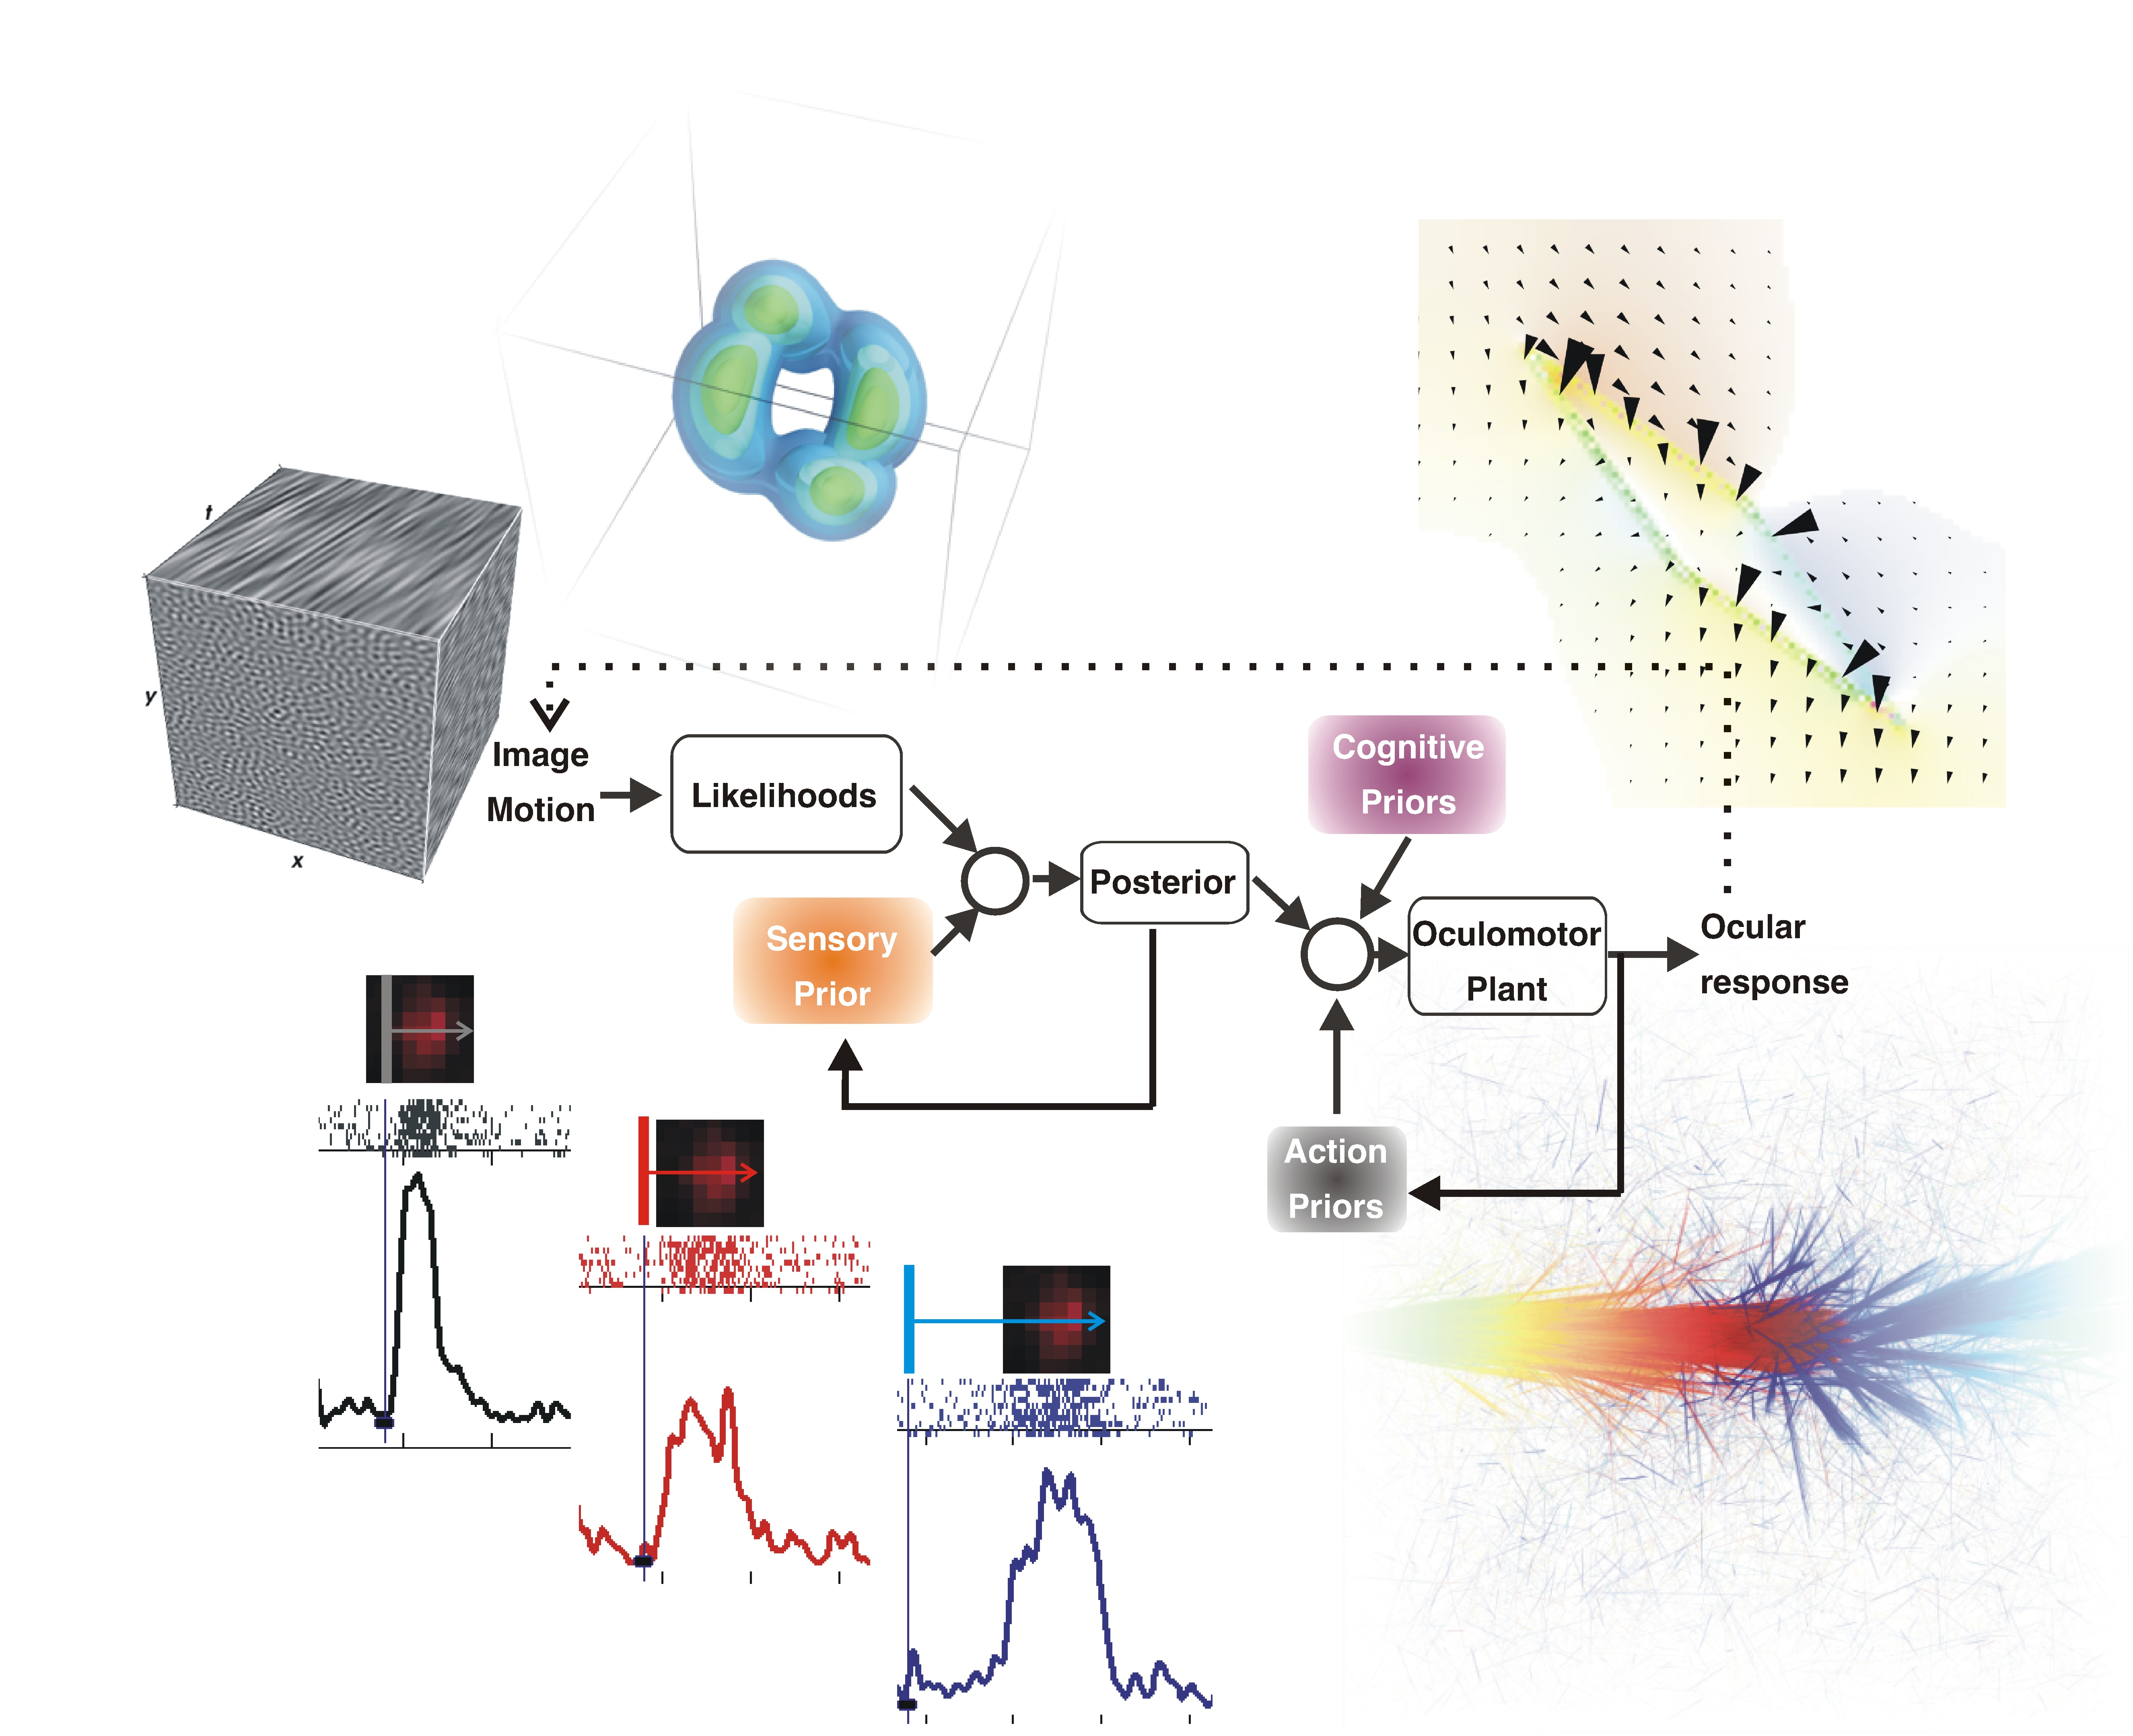
\includegraphics[width=1.\linewidth]{Inference_Ivibe5.jpg}}
%\caption{\textbf{Thématiques de recherche de l'équipe {\sc inViBe}:} L'équipe {\sc inViBe}, crée en 2010 vise à étudier différentes approches sur les mécanismes inférentiels qui sous-tendent la réponse comportementale dans le système oculomoteur. Ce schéma représente les différents aspects qui sont étudiés de la psychophysique~\citep{Sanz12} (cube en haut à gauche), aux modèles~\citep{Tlapale10,Perrinet12pred} (à droite) et à la physiologie par enregistrements extra-cellulaires de neurones de V1 analysés par Giacomo Benvenutti (en bas à gauche). Les modèles inférentiels de type Bayesien ici représentés par le modèle de \citet{Montagnini07}, constituent une synergie pour rassembler les différentes facettes présentes dans l'équipe. }%
%\label{fig:invibe}%
%\end{figure}%
%% - - - - - - - - - - - - - - - - - - - - - ----------------------------------------------- - - - - - - - - - - - -


%À ce titre, j'organiserai cette section autour des publications les plus représentatives.

% new team
En effet, suivant la restructuration des neurosciences sur les différents sites du CNRS à Marseille, le laboratoire INCM a intégré un nouveau site sur le campus de la faculté de médecine de la Timone, l'Institut de Neurosciences de la Timone (INT). Ce déménagement a pris place fin 2010 et a donné lieu à une restructuration des équipes arrivantes pour assurer la cohésion de l'ensemble. Notamment, l'équipe DyVA est devenue l'équipe ``inference and visual behavior'' ({\sc InViBe}). Tout en gardant de nombreux points commun avec les thèmes et méthodes développés à l'INCM, la formation de cette nouvelle équipe a permis de redéfinir son champ d'action. Notamment, l'accent a été mis sur l'intégration des pistes de recherche développées individuellement dans l'équipe et je vais développer dans cette section les principales contributions que j'ai pu apporter. %

% contrats : structuration / collaborations
Une étape importante dans la structuration du thème de recherche a été la recherche de nouvelles sources de financement et de nouvelles collaborations. En particulier, nous avons obtenu un financement important grâce au projet BrainScaleS (commission européenne, contrat numéro FP7-269921), qui nous a permis d'envisager l'élaboration de nouveaux types d'algorithmes basés sur ces recherches. Une autre étape importante a été la collaboration avec Karl Friston à l'University College de Londres qui a permis d'étendre la portée théorique des modèles probabilistes que nous utilisions. Cette collaboration a pris la forme d'une mission longue de 14 mois (d'octobre 2010 à février 2012) sous l'invitation de Karl Friston et a permis l'établissement de nombreuses collaborations dans Londres et nationalement (notamment Jim Bednar à Edinburgh). Ces différents facteurs ont contribué à la restructuration du projet de recherche durant cette période que je détaille ici.%

% plan de cette section: introduire les papiers pour la partie détaillée
%Dans cette section, je vais résumer les principaux axes de recherches qui ont été développés durant cette période.
En particulier, tout en gardant une lecture proche des niveaux d'étude de Marr, nous allons progressivement les dépasser pour mettre en avant les collaborations entre différents niveaux. Pour cela nous allons d'abord étudier une approche héritée de l'ingénierie des systèmes pour caractériser le système oculomoteur (Sec.~\ref{sec:motionclouds}), pour ensuite étudier le rôle fonctionnel des interactions latérales dans l'intégration spatio-temporelle, et en particulier le rôle du codage prédictif (Sec.~\ref{sec:prediction} et~\ref{sec:PerrinetBednar15}). Afin de confronter de tels modèles avec des données physiologiques et comportementales, nous allons enfin montrer des modèles de réseaux neuraux impulsionnels à grande échelle, tout en formalisant une théorie de décodage de cette activité neurale en terme d'information visuelle (Sec.~\ref{sec:spikes}). Enfin, nous synthétiserons ces différentes approches en présentant le modèle de minimisation de l'énergie libre présentée par Karl Friston et son application à l'unification des différentes théories qui ont cours en neurosciences computationnelles (Sec.~\ref{sec:free}).

\subsection{Caractérisation fonctionnelle du système oculomoteur~\citep{Sanz12,Simoncini12}}%
\label{sec:motionclouds}
Mesurer la vitesse et la direction d'un objet en translation est une étape computationnelle cruciale pour bouger nos yeux, nos mains dans l'environnement, attraper un objet ainsi que percevoir l'organisation de la scène visuelle et de ses éléments. Par exemple, alors que nous avons une bonne connaissance des mécanismes perceptifs et neuronaux de l'encodage et du décodage de l'information de direction ainsi que des algorithmes biologiquement plausibles utilisés dans différentes espèces, comment le cerveau traite et représente l'information de vitesse reste largement incompris. Des neurones sélectifs à la vitesse ont été identifiés à différents niveaux hiérarchiques des voies visuelles chez l'homme et le singe mais ne savons toujours pas précisément comment cette sélectivité est construite. Ceci explique l'absence de modèle consensuel sur cette question. Une hypothèse de travail est que ces mécanismes neuronaux, et leurs corrélats perceptifs, combinent de façon non-lineaire l'information locale de mouvement extraite à travers plusieurs filtres spatiotemporels, prenant avantage de la structure multi-échelle des images naturelles. De plus, l'organisation perceptive de la scène et de ses parties doivent être pris en compte pour une intégration contextuelle et dépendant de la tâche. Enfin, le code neural sous-jacent à la perception de la vitesse reste lui aussi largement mystérieux et donc nous sommes loin de comprendre comment l'information de vitesse est décodé pour contrôler des réponses (oculo-)motrices et des jugements perceptifs. Récemment, nous avons proposé que l'estimation de la vitesse est intrinsèquement un problème multi-échelle et dépendant de la tâche~\citep{Simoncini12}. Nous avons défini un nouveau type de stimulus visuel de mouvement, des textures dynamiques dont la phase est aléatoire. Ces stimuli possèdent plusieurs des propriétés statistiques des images naturelles~\citep{Sanz12,Vacher15nips}.


% - - - - - - - - - - - - - - - - - - - - - ----------------------------------------------- - - - - - - - - - - - -
%: figure MC artwork
\begin{figure}%
\centerline{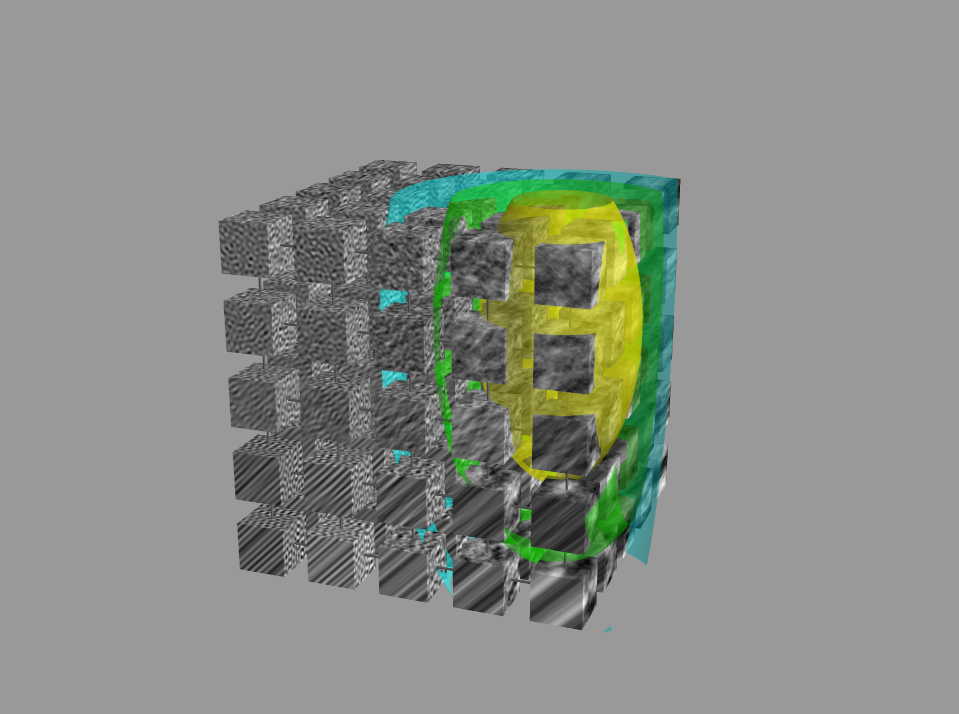
\includegraphics[width=.9\linewidth]{MCartwork.png}}
\caption{\textbf{Motion Clouds.} Les \emph{Motion Clouds}  (voir \url{https://neuralensemble.github.io/MotionClouds/}) constituent un ensemble de stimuli visant à explorer de manière systématique la réponse fonctionnelle d'un système sensoriel à un stimulus en mouvement de type naturel. Ceux-ci sont optimisées pour décrire un mouvement de translation pure en plein champ et sont par construction des textures synthétisées à partir de ``patchs" élémentaires de mouvement semblable placés au hasard dans l'espace~\citep{Sanz12,Vacher15nips}. L'objet de cet axe de recherche était de tester systématiquement le système visuel en variant les paramètres de telles textures sur les dimensions perceptives principales (vitesse moyenne, direction, l'orientation spatiale et fréquence). Nous montrons ici un \emph{espace de stimuli} comme une grille tri-dimensionnelle dont les n\oe dus correspondent à des stimuli et les axes des paramètres du mouvement: bande passante pour la vitesse (panneau de gauche), fréquence (panneau de droite) et orientation (partie supérieure). Chaque n\oe ud contient un cube élémentaire qui représente le film correspondant au stimulus, avec le temps qui s'écoule du coin inférieur gauche au coin en haut à droite dans les facettes à droite et en haut. Nous avons superposé en couleur une teinte qui représente une mesure de la réponse sensorielle (ici un modèle d'énergie du mouvement) dans cet espace de stimuli. Ce genre de caractérisation permet une étude systématique du système (ici oculomoteur) qui est étudié.
 }%
\label{fig:motionclouds}%
\end{figure}%
% - - - - - - - - - - - - - - - - - - - - - ----------------------------------------------- - - - - - - - - - - - -
%----------------------------------------------------------------------------------------------------------------
%motion clouds: kesako /
Une étape fondamentale a été franchie en important dans nos méthodes une approche héritée de l'ingénierie des systèmes. En effet, il est usuel pour caractériser le système oculomoteur d'utiliser des stimuli visuel simples comme des points, lignes ou des réseaux et de varier les paramètres de ces stimuli (contraste, orientation, direction, vitesse) pour en déduire la réponse comportementale. L'avantage de cette méthode est clairement la simplicité des stimuli. Toutefois, celle-ci s'accompagne paradoxalement avec le désavantage de créer des stimuli pour lesquels l'information peut être distribuée à différents niveaux de complexité structurelle. Ainsi une ligne en mouvement apporte un signal simple de mouvement, mais inclut intrinsèquement aussi des informations de haut niveau, comme l'alignement des différentes informations locales de mouvement. Une approche inverse est d'utiliser des stimuli écologiques en utilisant cette fois-ci des scènes naturelles. Le désavantage de ces stimuli est cette fois-ci que la complexité du stimulus est trop grande alors que l'on ne contrôle pas le contenu informationnel. Une solution pour caractériser le système oculomoteur est plutôt de faire l'hypothèse qu'il infère le mouvement d'un objet à partir d'un modèle interne de ce mouvement. En paramétrisant ce modèle, on peut générer grâce au modèle direct des stimuli qui seront optimaux pour caractériser le système ---sous réserve des hypothèses formulées. %

% Sanz12 / Simoncini
J'ai formalisé un tel modèle de génération de texture qui a ensuite été implanté pour l'étude de la détection du mouvement~\citep{Sanz12}, les \emph{Motion Clouds} (voir \url{https://neuralensemble.github.io/MotionClouds/}). Il s'appuie sur la formalisation la plus simple d'un détecteur élémentaire de mouvement, le modèle ``Motion Energy''~\citep{Adelson85}. Ce même modèle peut être de la même façon considéré comme la solution du problème inverse au modèle de conservation de la luminosité qui est souvent utilisé en vision par ordinateur~\citep{Aubert00}. Nous avons ensuite formulé ce modèle sous la forme d'un texture à phases aléatoires~\citep{Galerne10} en paramétrisant des axes perceptifs saillants (vitesse, direction, orientation) ainsi que les largeurs de bande (variabilité) qui leur sont associées (voir Fig.~\ref{fig:motionclouds}). On obtient alors des stimuli aux statistiques proches des images naturelles, avec un jeu de paramètres à contrôler et avec une implantation simple\footnote{Le code de cet algorithme de génération de textures est disponible sur \url{https://github.com/NeuralEnsemble/MotionClouds}.}. Grace à ce type de stimuli, nous avons pu par exemple caractériser la réponse oculomotrice en fonction de la richesse du contenu fréquentiel. Cette étude, parue dans \emph{Nature Neuroscience} (impact factor 16.7), nous a permis de dissocier les différents processus non-linéaires en jeu dans une tache décisionnelle ou perceptive: L'estimation du mouvement est intrinsèquement un problème multi-échelle et dépendant de la tâche~\citep{Simoncini12} (voir Fig.~\ref{fig:simoncini12}). Ces Motion Clouds constituent une base pour l'intégration de différentes études aux niveaux de la modélisation (pour valider les résultats théoriques), et aux niveaux physiologiques et comportementaux. %

En particulier, nous avons développé autour de cet ensemble de stimuli différents axes de recherche. Dans une première étude, en collaboration avec Andrew Meso et Guillaume Masson, nous avons étudié l'estimation de la vitesse en fonction du contenu fréquentiel de la texture. Cette tâche est importante car elle nous permet de dissocier les contributions indépendantes des différents canaux dans la hiérarchie des voies visuelles et ainsi de caractériser finement la dynamique de l'intégration spatio-temporelle. Les résultats de psychophysique indiquent l'importance d'une information a priori telle que prédite par des modèles Bayesiens~\citep{Stocker06}. De façon plus surprenante, nous observons aussi des phénomènes de sur-estimation de la vitesse qui peuvent être expliqués en complétant ce dernier modèle~\citep{Meso13vss,Meso14vss,Vacher15nips}. Ces résultats expérimentaux peuvent être expliqués de façon globale en modélisant l'ensemble des transformations visuelles.
En modélisant la génération aléatoire de  textures en trois dimensions transformées par des opérations géométriques telles que des rotations, des zooms et des translations nous avons expliqué l'émergence d'a priori probabilistes qui nous ont permis de valider ces hypothèses de façon expérimentale. C'est travaux ont été publiés dans une conférence à au niveau scientifique~\citep{Vacher15nips} et sont aussi publiés dans une revue à comité de lecture~\citep{Vacher16}.

%Dans une seconde étude, en collaboration avec Claudio Simoncini, Anna Montagnini, Laurent Goffart et Guillaume Masson, nous avons étudié le rôle du contenu fréquentiel des Motion Clouds sur les saccades de fixation. En effet, l'origine fonctionnelle de ces mouvements de faibles amplitudes est encore largement inconnu. En mesurant ces mouvements avec différentes classes de Motion Clouds, nous avons par exemple mis en évidence que certains aspects de ces mouvements corrèlent avec la statistique des textures, indiquant une possible fonctionnalité exploratoire des mouvements micro-saccadiques~\citep{Simoncini13vss}. %,Masson13sfn
%%Humans and monkeys fixational saccades are scaled with the statistics of naturalistic visual scenes
%%AUTHOR BLOCK: *G. MASSON, C. SIMONCINI, J. QUINET, L. U. PERRINET, A. MONTAGNINI, L. GOFFART;
%%
%Cette approche est donc novatrice et pertinente pour étudier les propriétés non-linéaires de l'intégration de mouvement, dans un contexte de réponse motrice ou de jugement perceptif sur la vitesse.

Ce projet a réuni des psychophysiciens, des spécialistes du contrôle oculomoteur chez l'homme et des modélisateurs pour caractériser le système oculomoteur. Notre but est d'étendre le travail élaboré ensemble ces dernières années pour comprendre comment mouvements de poursuite et perception visuelle tirent avantage d'un traitement multi-échelle pour estimer le mouvement d'une cible. Nous poursuivons notre travail de conception mathématique de stimuli de haute dimensionnalité grâce à notre modèle génératif des images naturelles. Grâce à eux, nous recherchons comment la vitesse est encodé grâce à l'extraction de l'énergie de mouvement dans différents filtres spatiotemporels. En analysant les réponses motrices et perceptives, nous mettons ainsi en évidence les mécanismes non-linéaires (dépendance au contraste, superposition, supra-linéarité, précision...) sous-jacente à l'intégration des sorties de ces filtres et nous pouvons donc modéliser ces mécanismes dans une nouvelle version de notre modèle computationnel. Par exemple det tels stimuli ont récemment été utilisés sur la rétine de rongeurs~\citep{Ravello19}. De plus, nous avons testé notre hypothèse que dans les scènes naturelles, ces mécanismes non-linéaires augmentent la précision des réponses et diminuent leur variabilité d'un essai à l'autre, ce qui conduit à des réponses motrices optimales. En comparant ces réponses motrices avec les jugements perceptifs, nous avons pu mettre en évidence une seconde hypothèse de travail: ces calculs non-linéaires dépendent de la tâche et du contexte sensoriel ou sensori-moteur~\citep{Simoncini12}. En particulier, nous avons vu dans quelle mesure les structures géométriques des scènes visuelles sont décisives pour la perception, au-delà du seul calcul de l'énergie de mouvement qui est utilisée par les mouvements oculaires. %
% - - - - - - - - - - - - - - - - - - - - - ----------------------------------------------- - - - - - - - - - - - -
% figure showing the psycho and model CRFs
\begin{figure}%
\centerline{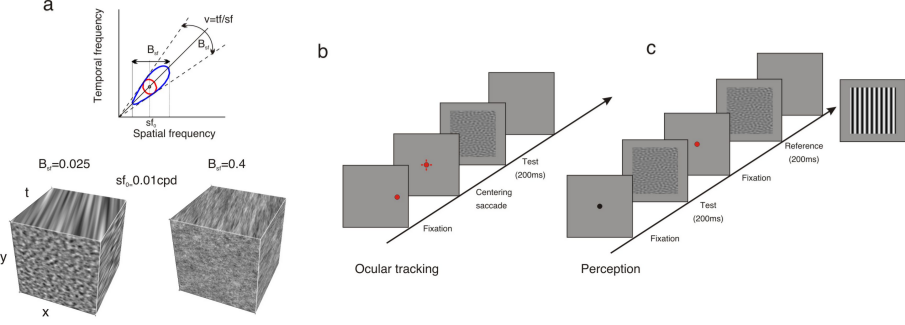
\includegraphics[width=\linewidth]{Simoncini12fig1.png}}
\caption{\textbf{Construction de stimuli de type Motion Clouds pour différentes tâches comportementales.} Pour montrer que l'estimation du mouvement est intrinsèquement un problème multi-échelle et tâche dépendant, nous avons construit le protocole suivant. (a) Dans l'espace représentant la distribution spatio-temporelle de fréquence (espace de Fourier), chaque ligne passant par l'origine correspond à des stimuli se déplaçant à la même vitesse. Un simple réseau en translation pure correspond à un seul point dans cet espace. Nos stimuli de texture en mouvement ont une énergie distribuée dans une ``ellipse''  allongée le long d'une ligne de vitesse donné, en gardant constantes les fréquences spatiales et temporelles moyennes. La bande passante spatio-temporelle a été manipulée par des largeurs de bandes différentes suivant ces axes, comme illustré par les cubes représentant les stimuli. La performance humaine a été mesurée pour deux tâches différentes, gérées en blocs parallèles. (b) Pour le suivi oculaire, les stimuli de mouvement ont été présentés pour une courte durée ($200~\ms$) à la suite d'un centrage saccadique, visant à contrôler à la fois l'attention et la précision de la fixation. (c) Pour la discrimination de la vitesse, des stimuli de test et de référence ont été présentés successivement pour la même durée et les sujets ont été invités à indiquer si le stimulus de test a été perçue comme lente ou plus rapide que la référence. Les résultats présentés dans~\citep{Simoncini12} montrent alors des effets opposés de la largeur de bande dans ces deux tâches. %
 }%
\label{fig:simoncini12}%
\end{figure}%
% - - - - - - - - - - - - - - - - - - - - - ----------------------------------------------- - - - - - - - - - - - -

\subsection{Rôle fonctionnel des interactions latérales dans l'intégration spatio-temporelle~\citep{Perrinet12pred,Khoei13jpp,KhoeiMassonPerrinet17}%
}%
\label{sec:prediction}%
%----------------------------------------------------------------------------------------------------------------
%: transport de prédiction: MCs = contrôle / ce qui nous intéresses c'est l'intégration (par exemple sur la trajectoire) / transport prédictif par filtre particulaire (nouveau soft à utiliser partout!)
Les Motion Clouds ne sont qu'une étape dans la construction d'une approche systémique de la caractérisation du système oculomoteur. Ceux-ci sont en effet construits sur des hypothèses simples de synthèse du mouvement et vont nous servir de contrôle: Les scènes naturelles se caractérisent en effet par de nombreuses régularités statistiques qu'il faut alors introduire dans le modèle génératif de synthèse du mouvement. En particulier, il est plus probable que la trajectoire de l'image d'un objet suive une trajectoire continue plutôt que dis-continue. Il est remarquable de noter qu'alors les modèles qui considèrent une indépendance conditionnelle entre les mesures voisines de mouvements considèrent par conséquent qu'une trajectoire dis-continue est aussi probable qu'une trajectoire continue.

Partant de ce constat, j'ai proposé un modèle d'intégration spatio-temporelle qui propose d'inclure l'information a priori que le mouvement d'un mouvement est continu et doit donc être pris en compte dans la dynamique globale du modèle. Nous avons mis en évidence la proximité de cette approche avec celle de~\citet{Burgi00} et aussi les limites de ce dernier modèle. En effet, établir des prédictions sur un espace de position et de vitesse entraine une explosion du nombre combinatoire de prédictions possible. À l'inverse du modèle précédent qui considère une approximation grossière de l'espace topographique de position et de vitesse, nous avons utilisé une technique de traitement de l'image appliquée au suivi de contours, les filtres particulaires. J'ai implanté un tel algorithme qui fournit ainsi une plateforme de modélisation que nous appliquons à différents problèmes.

Une première application de cette méthode a consisté à résoudre le problème de l'ouverture. En effet, ce problème est remarquable car il souligne qu'une information locale (par exemple le mouvement d'une ligne infinie) n'est pas suffisant pour caractériser le mouvement global (le mouvement d'un segment fini dans une direction non perpendiculaire à son orientation). Classiquement, il est établi que ce problème est résolu par des mécanismes spécialisés qui détectent soit le mouvement au centre du segment, soit le mouvement des fins de lignes. Alors, il est courant d'admettre que cette dernière information résout le problème de l'ouverture par un processus de compétition. Grâce au modèle de codage prédictif basé sur le mouvement, nous avons au contraire montré que ces mécanismes spécialisés étaient plutôt une propriété émergente du système: il est suffisant pour résoudre le problèmes de l'ouverture (voir Fig.~\ref{fig:perrinet12pred}).
% - - - - - - - - - - - - - - - - - - - - - ----------------------------------------------- - - - - - - - - - - - -
% figure showing the psycho and model CRFs
\begin{figure}%
\centerline{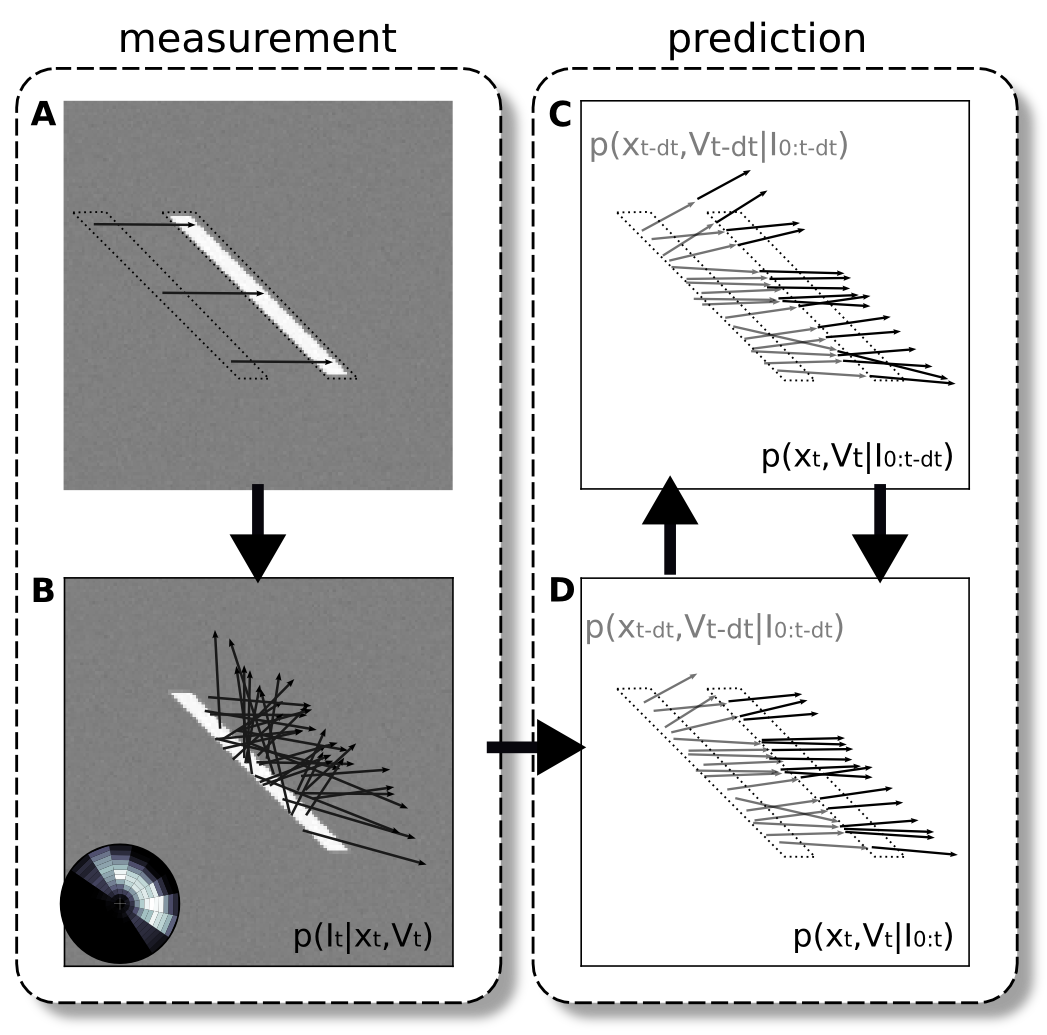
\includegraphics[width=\linewidth]{perrinet12pred_figure2.png}}
\caption{\textbf{Un codage prédictif basé sur le mouvement est suffisant pour résoudre le problème de l'ouverture.}
%The model is constituted by a classical measurement stage and of a predictive coding layer. The measurement stage consists of \textbf{(A)} inferring from two consecutive frames of the input flow, \textbf{(B)} a likelihood distribution of motion. This layer interacts with the predictive layer which consists of \textbf{(C)} a prediction stage that infers from the current estimate and the transition prior the upcoming state estimate and \textbf{(D)} an estimation stage that merges the current prediction of motion with the likelihood measured at the same instant in the previous layer (B).%
Ce modèle est constitué par un étage classique de mesure (estimation) et d'une couche de codage prédictif. L'étape de mesure consiste en \textbf {(A)} inférer à partir de deux trames consécutives du flux d'entrée \textbf {(B)} une distribution de probabilité de mouvement. Cette distribution est ici représentée par des échantillons dans l'espace possible des positions et vitesses du mouvement (flèches noires). Cette couche interagit avec la couche prédictive qui constitue \textbf {(C)} une étape de prédiction qui prédit l'état futur depuis l'estimation actuelle (des flèches grises aux flèches noires). Dans \textbf {(D)}, l'étape d'estimation fusionne la prévision actuelle de mouvement avec la probabilité mesurée au même instant dans la couche précédente (B), comme représenté par les flèches noires. %
Dans~\citep{Perrinet12pred}, nous avons montré qu'un tel modèle permet de résoudre le problème de l'ouverture. %
Ce même modèle a été étendu pour modéliser l'extrapolation du mouvement~\citep{Khoei13jpp} ou inclure des délais~\citep{KhoeiMassonPerrinet17}.
%
 }%
\label{fig:perrinet12pred}%
\end{figure}%
% - - - - - - - - - - - - - - - - - - - - - ----------------------------------------------- - - - - - - - - - - - -

%: extension avec motion extrapolation avec Anna Montagnini
Il est étonnant de constater qu'avec des hypothèses simples ---le codage prédictif basé sur le mouvement, nous pouvons ainsi caractériser des propriétés du système oculomoteur attribués classiquement à des mécanismes complexes et non-linéaires. Nous avons ainsi étendu, en collaboration avec Mina Khoei (en thèse FACETS-ITN) et Anna Montagnini (inViBe-INT), notre étude à un autre modèle classique pour l'oculomotricité: l'extrapolation du mouvement.
Cette extension consiste à étudier le comportement du modèle lors d'une interruption transiente de l'entrée sensorielle. En effet, il est courant ---par exemple lors d'un clignement de l'\oe il--- que l'entrée sensorielle soit perturbée ou suspendue, et il est important pour le système de représenter une certaine continuité. Celle-ci se traduit à partir de certaines étapes dans la hiérarchie du système visuel par une activité neurale soutenue pendant l'interruption, comme montré dans le cortex infero-temporal chez le macaque~\citep{Assad95}. Nous avons mis en évidence que notre modèle pouvait répliquer un tel comportement et en particulier, nous avons apporté trois points: 1) une prédiction à la fois en position et en vitesse est nécessaire pour avoir un comportement robuste, 2) la représentation du mouvement perd progressivement de sa précision lors de l'interruption, et 3) le système doit avoir accumulé assez d'information pour être dans un mode de suivi. Nous avons publié ces résultats dans différentes conférences et journaux~\citep{Khoei13jpp,KhoeiMassonPerrinet17}. Bien que ce modèle se base sur une conceptualisation de la propagation de l'information au sein d'une carte corticale (utilisant les filtres particulaires), nous verrons dans la section suivante (Sec.~\ref{sec:spikes}) qu'elle admet une implantation neuromimétique.

\subsection{Rôle fonctionnel des interactions latérales dans l'intégration spatiale~\citep{PerrinetBednar15}%
}%
\label{sec:PerrinetBednar15}%

%: champ associatif avec Bednar= autre direction (dans l'espace pas le temps)
En parallèle de l'étude de la prédiction spatio-temporelles nous avons concentré nos efforts sur les dépendences spatiales dans les images naturelles.
En effet, un autre axe d'exploration est d'implanter un prior d'association local similaire à celui utilisé pour le codage prédictif dans le temps (basé sur le mouvement), cette fois en étudiant les régularités statistiques des scènes naturelles dans l'espace à un instant donné. Une telle tâche est similaire à l'identification d'un ``champ associatif" qui connecterait des neurones sélectifs à des orientations locales suivant leur régularités~\citep{Field93}. Ce concept est controversé car les études qui ont montré un corrélât neural pour une telle connectivité~\citep{Bosking97} sont souvent en contradiction avec des études physiologiques~\citep{Chavane11,Hunt12}. En collaboration avec Jim Bednar (DTC, Edinburgh), j'ai utilisé des travaux précédents sur le représentation en ondelettes~\citep{Fischer07cv} pour quantifier un tel champ associatif. Il en ressort deux traits principaux: 1) quand on mesure la probabilité de cooccurrence de deux contours (voir Figure~\ref{fig:PerrinetBednar15}), leurs propriétés absolues (échelle, distance) sont indépendant de leur propriétés géométriques (azimuth, angle relatif); 2) les propriétés géométriques sont suffisantes pour caractériser des propriétés de ces images comme par exemple leur catégorie (animal/ non-animal ou naturel / artificiel). Nous avons détaillé ces résultats dans un publication dans le journal Scientific Reports~\citep{PerrinetBednar15}. Ces axes de recherche ---prédiction sur une trajectoire et dans l'espace--- sont complémentaires et nous verrons dans mon programme de recherche qu'il est possible de les combiner.

% - - - - - - - - - - - - - - - - - - - - - ----------------------------------------------- - - - - - - - - - - - -
%% figure showing the psycho and model CRFs
\begin{figure}%
\centerline{%
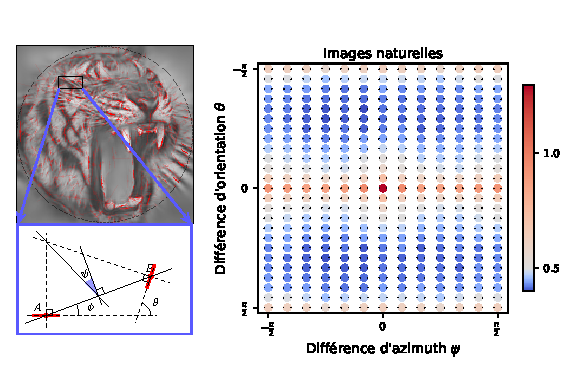
\includegraphics[width=\linewidth]{figure_synthesis_FR.pdf}
}
\caption{
\textbf{Co-occurrences de bord}:
 (A) Exemple d'image avec la liste des bords extraits superposés. Chaque arête est représentée par un segment de ligne rouge qui représente sa position (centre du segment), son orientation et son échelle (longueur du segment). Nous avons contrôlé la qualité de la reconstruction à partir de l'information de bord de sorte que l'énergie résiduelle était inférieure à 5\%. (B) La relation entre un bord de référence «A» et un autre bord «B» peut être quantifiée en fonction de la différence entre leurs orientations $\theta $, le rapport de l'échelle $\sigma $, la distance $ d $ entre leurs centres, mais aussi la différence d'azimuth $\phi $. De plus, nous définissons $\psi =\phi -\theta / 2 $, qui est symétrique par rapport au choix du bord de référence; En particulier, $\psi = 0 $ pour toute arêtes co-circulaires. Comme dans~\citet {Geisler01}, les arêtes en dehors d'un masque circulaire central sont rejetées dans le calcul des statistiques pour éviter les artefacts.
%
 }%
\label{fig:PerrinetBednar15}%
\end{figure}%
% - - - - - - - - - - - - - - - - - - - - - ----------------------------------------------- - - - - - - - - - - - -

% communiqué INSB http://www.cnrs.fr/insb/6.recherche/parutions2/articles2015/l-perrinet.html
%
%
%
%En modélisant notre capacité à distinguer un animal dans une scène visuelle, des chercheurs de l?Institut de neurosciences de la Timone et de l?Université d'Edinburgh lèvent le voile sur certains des mystères de la perception visuelle. Ils démontrent que la classification très rapide par le cerveau d?une image contenant ou non un animal, est possible à un niveau de représentation relativement primitif à partir de régularités statistiques simples, et non, comme cela est généralement admis, après une longue série d'analyses visuelles de plus en plus abstraites. Cette étude est publiée dans la revue Scientific Reports.
%
%
%Classifier une image, par exemple en décidant si elle contient ou non un animal, est une des fonctions de base du cerveau. Dans le royaume animal, on comprend aisément qu?elle constitue une fonction vitale aussi bien pour des prédateurs que pour leurs proies. Les mécanismes sous-jacents sont de plus en plus étudiés aussi bien dans le domaine des systèmes d'intelligence artificielle que dans celui des Neurosciences, mais ils restent encore bien mystérieux pour les chercheurs. En effet, si les réseaux d'ordinateurs les plus avancés peuvent aujourd'hui aisément calculer numériquement des quantités phénoménales de données à partir de bases de données pharaoniques, même les systèmes les plus avancés de classification d'images n'égalent pas encore les capacités d'un jeune enfant!
%
%Laurent Perrinet de l?Institut de Neurosciences de la Timone à Marseille et James Bednar de l?université d'Edinburgh en Écosse, ont modélisé la façon dont nous pouvons classer différentes catégories d'images. Leur l'objectif initial était de différencier des scènes visuelles naturelles de scènes d'intérieur, mais ils ont pu montrer que ce système simple de classification permettait aussi de détecter en une fraction de seconde des animaux dans une image. En effet, ils ont mis en évidence qu'un niveau de performance comparable à celui d?observateurs humains est atteignable tout en utilisant un niveau de représentation très primitif, et non, comme cela est généralement admis, après une longue série d'analyses visuelles de plus en plus abstraites (détection des yeux et des membres, puis de la tête et du corps, etc...).
%
%Cette représentation primitive se base sur les modèles existants de représentation des images dans les aires visuelles de bas niveau des primates. On estime en effet que dans le cortex visuel primaire les images visuelles sont représentées dans l'activité neurale comme l'organisation de contours élémentaires, à la manière d?un peintre qui dessine une silhouette en une série de coups de pinceau. Une des innovations majeures dans cette étude consiste à simplement utiliser la fréquence des configurations entre des paires de contours élémentaires comme représentation d'entrée utilisée pour le classificateur.
%
%Pour arriver à ce résultat, les chercheurs ont utilisé des modèles mathématiques de la représentation des images dans le cortex visuel primaire et en particulier les inter-relations entre des éléments de contours voisins. En étudiant les résultats de l'analyse, on note que dans les images naturelles, des contours parallèles sont observés majoritairement, signe que les contours et textures présents dans les images contiennent en majorité des alignements. C'est encore plus vrai dans les environnements artificiels comme dans une scène d'intérieur (par exemple un bureau) où les bords francs dominent. On montre aussi que les objets co-circulaires (c'est-à-dire des configurations symétriques) sont aussi relativement plus présents que des configurations aléatoires.
%
%La principale nouveauté de cette étude est de montrer que les images contenant un animal (quelle que soit son espèce ou sa position dans l'image) contiennent sensiblement plus de configurations symétriques. Cette différence suffit pour expliquer le niveau de performance de classification chez les humains quand on leur présente de telles scènes de façon très brève.
%
%Pour valider cette hypothèse, les chercheurs ont alors utilisé des données précédemment enregistrées dans lesquelles des volontaires regardaient et classifiaient des centaines d'images. En utilisant cette représentation primitive, ils ont mis en évidence qu'un programme très simple pouvait facilement classifier les images comme contenant ou non un animal, sans avoir besoin d?une connaissance plus élaborée sur les caractéristiques de l?animal comme sa position, sa taille ou son orientation sur l?image.
%
%Cette découverte peut accélérer le développement de requêtes via des images dans les moteurs de recherche, comme Google et Facebook, car elle permet une classification simple et robuste grâce à des caractéristiques statistiques de bas niveau basées sur la géométrie des objets. Elle pourrait ainsi améliorer l'efficacité de tels algorithmes. Toutefois, et comme cela a été mis en évidence dans la psychophysique humaine, les catégories visuelles doivent être visuellement assez distinctes: ce traitement rapide ne permet pas, par exemple, de distinguer une scène de montagne d'une scène de mer. De manière surprenante, les chercheurs ont montré que lorsque les humains se trompent en classifiant de manière erronée une image comme contenant un animal, le programme a tendance à se tromper de la même façon! En utilisant des modèles mathématiques, on peut donc imaginer synthétiser des images d'animaux qui en fait, n'en contiendraient pas. Ces "chimères" seront sûrement très utiles pour percer encore plus les mystères du système visuel.
%
Dans le futur, l'extension de cette représentation calculée sur l'ensemble de l'image pourrait être améliorée en la couplant à des processus de classification locaux permettant de déterminer par exemple la position de l'objet à classifier et de segmenter progressivement la figure du fond afin de diminuer ainsi les distractions.

\subsection{Modélisation de réseaux de neurones impulsionnels}%~\citep{Taouali15}
\label{sec:spikes}
L'étude que nous menons sur les régularités statistiques ---dans les trajectoires des objets et dans l'espace--- se doivent d'être validés par les résultats expérimentaux. Pour ce faire, nous utilisons deux approches complémentaires. La première consiste à utiliser des simulations à grande échelle des conductivités que nous avons mis en évidence pour comprendre si ces principes s'étendent tels quels à des réseaux de neurones. La deuxième approche consiste à utiliser les données neurales collectées au laboratoire et d'utiliser nos modèles pour décoder de l'activité neurale l'information visuelle pertinente.

%: modélisation avec Lansner et Kaplan / anisotropic = novel /
Dans le premier axe, nous avons implanté en collaboration avec Bernhard Kaplan, Anders Lansner (KTH, Suède) et Frédéric Chavane (inViBe-INT), et dans le cadre de BrainScaleS, des simulations à grande échelle d'une aire corticale implantant le codage prédictif basé sur le mouvement. Cette simulation est basée sur le savoir-faire du KTH en la matière et nous a permis de valider le modèle probabiliste à l'échelle neuro-morphique. Nous avons utilisé comme contrôle le protocole d'extrapolation du mouvement (voir plus haut et~\citep{Khoei13jpp}). Les résultats ont montré des résultats similaires aux résultats théoriques (notamment les trois points évoqués plus haut), ainsi qu'une propriété reliée à l'implantation neurale. Durant l'interruption, la représentation probabiliste au niveau de la population de neurones reste la même, mais le niveau d'activité global (en termes de fréquence de décharge) diminue, en accord avec par exemple les mesures dans le cortex infero-temporal chez le macaque~\citep{Assad95}. Nous avons détaillé ces résultats dans une publication commune~\citep{KaplanKhoei14}. Il est important de noter que ce type d'implantation est basé sur une connectivité anisotropique qui n'avait jamais ---à notre connaissance-- été explorée. Ce modèle a fait partie des modèles sélectionnés dans BrainScaleS pour être implantés finalement sur les micro-circuits neuromorphiques à grande échelle.

%: décodage (avec Giacomo)
%\subsection{Spiking Motion Extrapolation}
Un aspect complémentaire à la simulation est l'étude du décodage de l'activité neurale. En collaboration avec Giacomo Benvenutti (thèse BrainScaleS) et Frédéric Chavane (inViBe-INT), nous avons étudié des modèles statistiques qui nous permettent d'extraire l'information visuelle de populations de neurones. En premier lieu, une telle approche permet de consolider les bases théoriques qui permettent de caractériser l'activité neurale, tant au niveau de la statistique de fréquence de tir des neurones que pour la paramétrisation des courbes de sélectivité neurale, par exemple en fonction de l'orientation et de la direction. Aussi, une telle caractérisation nous permettent de valider des modèles de décodage et de représentation de l'information dans l'activité neurale (comme par exemple~\citep{Jazayeri06}) et ainsi de boucler le lien avec l'implantation neurale de tels processus. %

Pour ce faire nous avons recruté une étudiante en post doctorat, Wahiba Taouali, pour mieux comprendre les fondements mathématiques du décodage neural. Une première tâche a consisté à quantifier les différentes sources de bruit dans les enregistrements neurophysiologiques obtenus au laboratoire. En particulier, nous avons développé une méthodologie mathématique permettant de caractériser la variabilité des trains de potentiels d'action. Ce test statistique novateur nous a permis de montrer que la variabilité intrinsèque aux enregistrements s'établissaient de façon différentielle de la rétine, au thalamus et aux aires corticales supérieures. Ces travaux on fait l'objet d'une publication dans un journal à comité de lecture~\citep{Taouali16}.

Une fois que ces principes du codage neural étaient mieux compris, nous les avons appliqués à des enregistrements effectués dans le cortex visuel primaire  évoqué par une barre en mouvement. Grâce à la méthode de décodage neural nous avons pu valider l'hypothèse selon laquelle dans la représentation neurale, une population de neurones peut coder de façon efficace la position et l'orientation d'une barre en mouvement. En particulier, une signature particulière du codage neural montre qu'une barre en mouvement selon une trajectoire prédictive anticiper le long de son mouvement~\citep{Taouali15vss,Taouali16areadne,Perrinet19nccd}. %Ces travaux sont en cours écriture pour une publication dans un journal à comité de lecture.

%
\subsection{Unification des théories computationnelles par la minimisation de l'énergie libre (MEL)~\citep{PerrinetAdamsFriston14} }
\label{sec:free}
%%%%%%%%%%%%%%%%%%%%%%%%%%%%%%%%%%%%%%%%%%%%
%: figure 0
\begin{figure}%[ht]%
\begin{center}
%  \makebox[\textwidth]{
   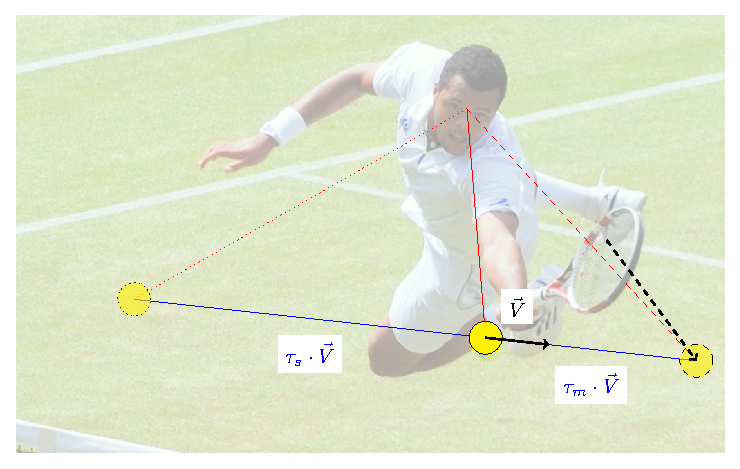
\includegraphics[width=\columnwidth]{figure-tsonga}%friston_figure0.pdf}%
%  }%
\end{center}%
\caption{%
%Problem statement: optimal motor control under axonal delays. The central
%nervous system has to contend with axonal delays, both at the sensory and the
%motor levels. For instance, in the human visuo-oculomotor system, it takes
%approximately $\tau_s=50~\ms$ for the retinal image to reach the visual areas
%implicated in motion detection, and a further $\tau_m=40~\ms $ to reach the
%oculomotor muscles. As a consequence, for a tennis player trying to intercept a
%ball at a speed of $20~\m\cdot \s^{-1}$, the sensed physical position is $1~\m$
%behind the true position (as represented here by $\tau_s \cdot \vec{V}$), while
%the position at the moment of emitting the motor command will be $.8~\m$ ahead
%of its execution ($\tau_m \cdot \vec{V}$). Note that while the actual position
%of the ball when its image produced by the photoreceptors on the retina hits
%visual areas is approximately at
%$45$ degrees of eccentricity (red dotted line), the player's gaze is directed to
%the ball at its \emph{present} position (red line), in anticipatory fashion.
%Optimal control directs action (future motion of the eye) to the expected
%position (red dashed line) of the ball in the future --- and the racket (black
%dashed line) to the expected position of the ball when motor commands reach the
%periphery (muscles).
La commande motrice doit être optimale sous la contrainte de délais axonaux. En effet, le système nerveux central doit faire face aux retards axonaux, tant au niveau sensoriel que moteur. Par exemple, dans le système visuo-oculomoteur humain, il faut environ $\tau_s = 50 ~\ms $ pour que l'image rétinienne atteigne les zones visuelles impliquées dans la détection de mouvement, et encore $\tau_m = 40 ~\ms $ pour atteindre les muscles oculomoteurs. En conséquence, pour un joueur de tennis qui essaie d'intercepter une balle  à une vitesse de $ \vec {V} = 20 ~\m\cdot\s ^ {- 1} $, la position physique détectée est en fait à environ $ 1 ~\m $ derrière la position vraie (comme représenté ici par $\tau_s\cdot\vec {V} $), alors que la position au moment de l'émission de la commande motrice se situera à $ .8 ~\m $ après son exécution ($\tau_m\cdot\vec {V} $). Notez qu'à cet instant, si la position réelle de la balle donnée par son image visuelle transmise par les photorécepteurs de la rétine  est approximativement à $ 45 $ degrés d'excentricité (ligne pointillée rouge), le regard du joueur est dirigé vers la balle à sa position \emph{présente} (ligne rouge), de façon anticipée. Un contrôle optimal commande l'action (le mouvement futur de l'\oe il) de cette position retardée de la balle dans l'avenir --- vers celle de la raquette (ligne noire brisée) pour diriger l'action vers la position attendue de la balle lorsque l'action atteint la périphérie (muscles).
}%
% warn perhaps about the notion of interception
% another ecological example if when the subjzct is moving
\label{fig:figure0}
\end{figure}
%%%%%%%%%%%%%%%%%%%%%%%%%%%%%%%%%%%%%%%%%%%%

% - - - - - - - - - - - - - - - - - - - - - ----------------------------------------------- - - - - - - - - - - - -
% figure MEL de Friston10c
\begin{figure}%
\centerline{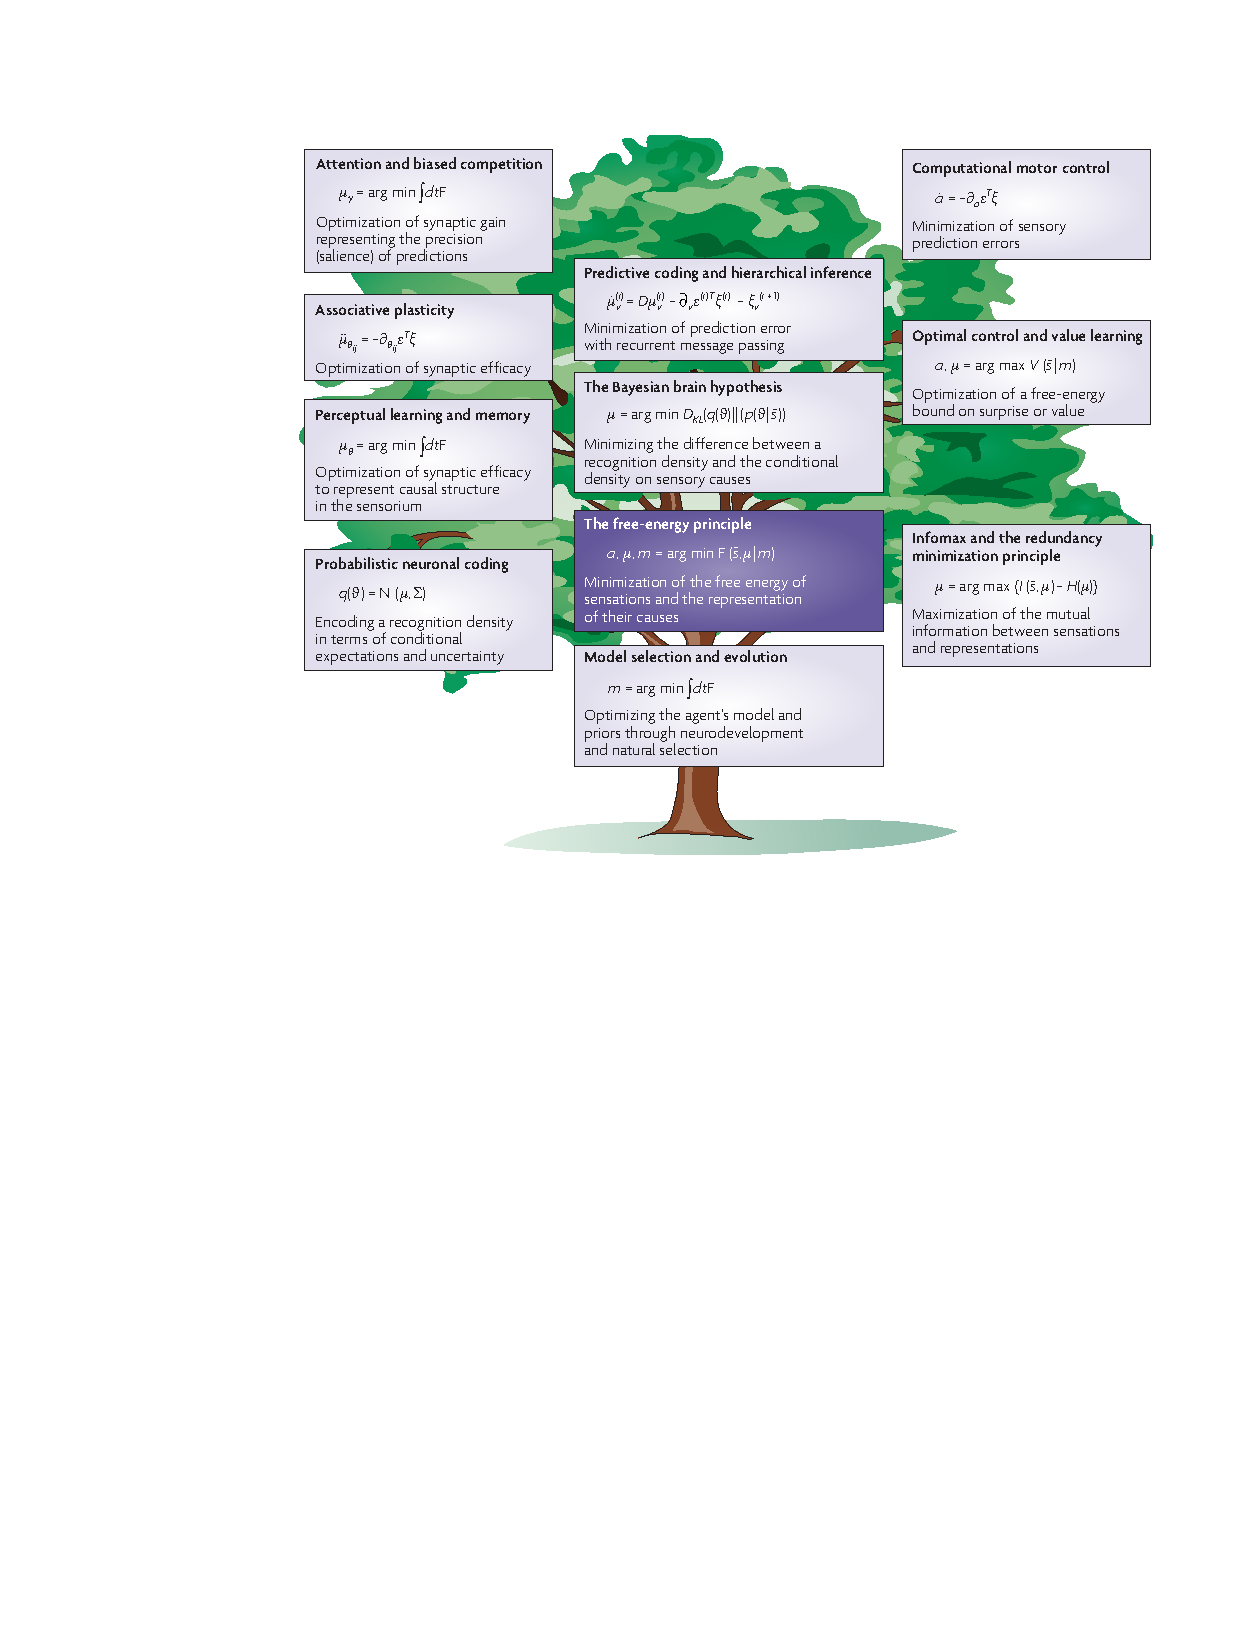
\includegraphics[width=\linewidth]{friston10c_fig4.pdf}}
\caption{\textbf{Unification des théories computationnelles par la minimisation de l'énergie libre (MEL).}
Cette figure extraite de~\citep{Friston10c} représente la place central du principe de MEL dans l'ensemble des théories computationnelles. En particulier, on peut noter que les principes que nous avons détaillés plus haut dans les chapitres précédents (réseaux de neurones heuristiques, principes d'optimisation, codage prédictif, ...) peuvent se rapporter à ce langage commun. %
 }%
\label{fig:friston10c_fig4}%
\end{figure}%
% - - - - - - - - - - - - - - - - - - - - - ----------------------------------------------- - - - - - - - - - - -
%: EL / MEL / novateur
L'énergie libre est une mesure statistique qui quantifie la surprise d'échantillonner des données (par exemple sensorielles), connaissant \emph{a priori} un modèle génératif de la synthèse (cause) de ces données. L'hypothèse de minimisation de l'énergie libre (MEL) considère que tout agent qui résiste à la tendance au désordre (tendance dictée par le second principe de la thermodynamique) développe alors nécessairement des stratégies de MEL, car celle-ci donne une borne supérieure mesurable de la surprise, c'est-à-dire de l'entropie liée à un modèle génératif. Dans la théorie développée par Karl Friston (UCL, Londres), appliquant ce principe aux neurosciences, il ajoute deux hypothèses supplémentaires:
\begin{itemize}
\item Le modèle génératif est hiérarchique et non-linéaire~\citep{Friston08b},
\item La représentation des données comme densité de probabilité est approchée par des lois normales (approximation Laplacienne) dont les moments sont explicitement codés dans la décharge neurale~\citep{Friston09a}.
\end{itemize}
Une première conséquence de ce principe est qu'un système appliquant ce principe modifie son état interne pour minimiser sa surprise. Cette minimisation s'établit aux différents niveaux du modèle hiérarchique et s'implante par la communication de transferts d'informations, généralisant ainsi la théorie établie par~\citet{Mumford92}. Cette jeune théorie, en plein développement théorique et applicatif, a engendré une unification ---parfois décriée--- de nombreux pans des approches computationnelles en neurosciences. Elle constitue à ce titre une avancée majeure dans les neurosciences dans ces dernières années.

%: mission longue / mes 3 papiers avec Friston /un détaillé ici
J'ai initié une collaboration avec Karl Friston en 2010 pour appliquer ce principe à la modélisation du système oculomoteur. J'ai réalisé cette collaboration au cours d'une mission longue entre octobre 2010 et février 2012. Durant cette période, j'ai intégré son équipe de neurobiologie théorique, développé un modèle unificateur pour le système oculomoteur que nous avons décliné dans un premier temps en trois projets: Dans le premier, nous avons étudié comment ce principe pouvait permettre de décrire les principes computationnelles de la recherche visuelle (visual search) en l'appliquant à un modèle de saccades oculaires~\citep{Friston12}. En parallèle, nous avons étudié dans un second papier comment un modèle de la poursuite lente pouvait expliquer des phénomènes observés chez des patients schizophréniques~\citep{Adams12}.

Ce travail a culminé avec la formalisation d'un modèle intégré du système oculomoteur. On particulier nous nous sommes attachés à prendre en compte l'existence d'inévitables délais de traitement entre la sensation rétinienne et la prise de décision oculo-motrice. L'inclusion de cette contrainte du système oculomoteur nous a permis le développement d'une théorie mathématique novatrice pour expliquer l'intégration du mouvement entre une sensation rétinienne retardée et le modèle interne. C'est travaux ont fait l'objet d'une publication dans le journal Biological Cybernetics~\citep{PerrinetAdamsFriston14} et de nombreuses applications notamment de pouvoir modéliser l'illusion du Flash retardé~\citep{KhoeiMassonPerrinet17}.

%: outlook: synthèse de ces différents niveaux / similarité avec l'approche systémique
La majeure innovation de ce principe est de considérer l'agent et son environnement de façon globale. Dans cette approche systémique, le système oculomoteur est considéré comme un système intégré plutôt que le chaînage de processus élémentaires de traitement comme ce qui est classiquement accepté~\citep{Robinson86,Krauzlis89}. Appliqué à un agent, c'est-à-dire à un système pouvant agir sur son environnement pour minimiser son énergie libre, le principe de MEL conduit à l'\emph{inférence active}~\citep{Friston09c}. Cette théorie permet d'unifier des modèles de natures différentes (probabilistes, modèle de contrôle, codage prédictif, réseaux Bayesiens, heuristiques sur des réseaux de neurones, ...) en proposant un langage commun~\citep{Friston10c} (voir Fig.~\ref{fig:friston10c_fig4}). Nous avons détaillé cette proposition dans une publication dans le journal Biological Cybernetics qui montre des exemples concrets de ces différentes approches sur l'application de ce principe~\citep{PerrinetAdamsFriston14}. %
%Je vais développer dans mon programme de recherche les extensions de ces travaux dans mes perspectives de recherche.

%
%
%%!TEX TS-program = PdfLaTeX
%%!TEX root = perrinet17cnrs.tex
%%!TEX encoding = IsoLatin
%%!TEX spellcheck = fr-FR
%\chapter{Objectifs \& Projet de recherche}
%\label{part:outlook}
%
%%\chapter{Perspectives de recherche}
%
%%Cette partie concerne uniquement les rapports à 10 semestres. Vous présentez :
%%les objectifs de vos recherches pour les 10 prochains semestres, en les mettant en perspective avec les objectifs de votre unité de recherche et à la politique scientifique du CNRS ;
%%et éventuellement vos objectifs concernant les autres facettes de votre activité :
%%- enseignement, formation et diffusion de la culture scientifique,
%%- transfert technologique, relations industrielles et valorisation,
%%- encadrement, animation et management de la recherche.
%
%Comme exposé dans mon rapport d'activité à 10 semestres (chapitre~\ref{chap:projet}, j'ai développé depuis mon intégration au CNRS une thématique étendue dans le domaine de l'étude du système oculomoteur en la focalisant sur l'axe du codage prédictif.
%J'ai présenté dans la partie précédente ces axes de recherche en développant en particulier mes axes de recherche actuels. Focalisons-nous maintenant sur quatre projets particuliers qui posent de façon détaillée les bases prospectives de mon projet de recherche:
%\begin{enumerate}
%\item Tout d'abord, dans le chapitre~\ref{sec:prediction}, nous avons exposé le modèle de codage prédictif basé sur le mouvement appliqué au problème de l'extrapolation du mouvement. Cette partie va définir un modèle de propagation anisotropique de l'information en le basant sur les méthodes de filtrage particulaire. Nous avons détaillé les résultats obtenus et leur signification au niveau des réponses comportementales.
%\item Ensuite, dans la section~\ref{sec:PerrinetBednar15}, nous avons étendu le codage prédictif en étudiant une quantification statistique du champ associatif. Pour montrer la puissance d'une telle représentation, nous l'avons utilisée pour classifier des images, comme par exemple des images contenant des animaux ou non. Cette démarche permet de montrer que ce champ associatif ---et donc un algorithme utilisant un modèle avec des interactions latérales--- permet de construire des algorithmes efficaces de traitement de l'information. Il se pose donc comme une alternative novatrice et complémentaire aux modèles hiérarchiques (de type apprentissage profond) et purement "en avant" qui sont couramment admis dans la littérature~\citep{Serre07}.
%\item Afin de valider à l'échelle neurale de tels algorithmes nous avons proposé dans le chapitre~\ref{sec:spikes} une implantation neurale du modèle décrit dans les sections précédentes. Les résultats montrent qu'un telle implantation n'est pas triviale et demande de définir de façon précise le micro-circuit qui implante au niveau de l'activité neurale les processus inférentiels décrits plus haut.
%\item Enfin, dans la section~\ref{sec:free}, j'ai développé la formulation de minimisation de l'énergie libre en l'appliquant au système oculomoteur simplifié, mais pris dans sa globalité. Nous nous sommes attaché en particulier au problème des délais sensori-moteurs dans ce système et avons proposé une méthodologie pour résoudre ce problème. Les résultats ont montré l'émergence de comportement attribués classiquement à des systèmes complexes et que nous pouvons ici décrire de façon économique grâce à la théorie formulée par Karl Friston.
%\end{enumerate}
%
%
%En utilisant ces quatre piliers, nous allons maintenant essayer de dégager les perspectives de recherche qui vont structurer mon programme de recherche futur. L'idée maitresse est (i) d'utiliser les contraintes biologiques (délais, resources limitées) comme des outils pour mieux comprendre le fonctionnement au niveau théorique (ii) d'appliquer ces outils théoriques à des problèmes pratiques, comme la robotique. Ceux-ci sont articulés autour de 3 projets: TRAX, AsyncDrone et ALELOM.%
%
%\section{TRAX: une théorie unifiée du traitement des trajectoires visuelles}
%
%
%Le mouvement des objets dans les scènes naturelles se fait principalement le long de trajectoires, c'est-à-dire suivant une séquence de positions cohérentes dans le temps par rapport à leur mouvement. Comment les systèmes sensoriels exploitent cette connaissance \emph{a priori} est une question majeure pour les neurosciences computationnelles et la vision par ordinateur. Imaginons un serpent nageant à la surface d'une rivière. Pour extraire et suivre son mouvement, il faut résoudre de difficiles problèmes d'estimation, rendus d'autant plus compliqués par la transparence de l'eau et la non-rigidité du corps du serpent. De plus, les capteurs de mouvement étant limités dans leur extension spatiale, ce corps longiligne peut faire apparaitre une ambiguité sur la vitesse, le \emph{problème de l'ouverture} (voir la section~\ref{sec:prediction}). Il existe de nombreuses solutions à ces problèmes aussi bien en vision par ordinateur qu'en neurosciences computationnelles. Une hypothèse centrale et novatrice du projet TRAX est le fait que le système visuel de bas niveau des mammifères peut les résoudre de façon hautement performante ---tant en termes d'acuité que de robustesse--- grâce à des micro-circuits génériques dont le réseau d'inter-connectivité implante la fonction visuelle et que des règles d'apprentissage adaptent de façon optimale la connectivité aux statistiques des scènes naturelles (voir Figure~\ref{fig:trax}).
%
%
%%------------------------------------------------------------------------------------------------%
%%: see Figure~\ref{fig:trax}
%\begin{figure}[b!]%[p!]%[p!] %h!]%
%\centering%
%\includegraphics[width=\textwidth]{led-lights-long-exposure-violin.png}
%
%\caption{\textbf{TRAX: poursuivre des trajectoires.} Cette image montre une image à longue exposition d'un violoniste sur lequel on a lixé des LEDs sur son archet [avec permission from \href{http://www.motionexposure.com/Galleries/ViolaViolin/i-CdTcF5V/A}{Stephen Orlando]}.
%Le mouvement complexe des points individuels exhibe un ensemble de trajectoires prototypiques du mouvement rigide d'un objet. Le répertoire de ces mouvements permet d'affiner des algorithmes de détection du mouvement en combinant cohérence spatiale et temporelle.
% } \label{fig:trax} %
%\end{figure} %
%%------------------------------%
%Ce projet fait actuellement l'objet d'un demande de financement avec des partenaires français (ENS). L'objectif global de ce projet est de fournir un cadre théorique unifié pour comprendre les transformations sensorielles opérant dans les aires corticales visuelles pour permettre d'extraire la trajectoire des contours. Les partenaires impliqués possèdent chacun une expertise forte en neurosciences computationnelles ou en vision par ordinateur, et sont tous spécialisés dans la compréhension des mécanismes de description de bas niveau des images. Nous allons faire collaborer ces chercheurs autour de cette question théorique centrale. Spécifiquement, nous nous centrerons sur l'aire visuelle primaire comme modèle générique de représentation pour les scènes visuelles sous forme de contours élémentaires, ceux-ci étant définis comme des chaines de bords orientés reliés par une probabilité de co-occurence significative. Nous étudierons conjointement les différents problèmes (segmentation, correspondance, ouverture) liés à cette tâche computationnelle pour faire émerger une approche unifiée. Une notion clé est que les trajectoires des contours dans les scènes naturelles suivent des courbes prototypiques que nous pouvons caractériser quantitativement. Nous pourrons alors exploiter ces statistiques pour calculer la probabilité de chaque co-occurence d'appartenir au même contour.
%
%Pour atteindre cet objectif, la méthode générale consiste à combiner les compétences des partenaires de ce projet en synergie autour de tâches progressivement plus ambitieuses. Premièrement, les statistiques des images naturelles vont nous permettre d'affiner un modèle génératif de synthèse de textures. Ce modèle pourra alors servir d'algorithme dans le processus de détection de contours, mais aussi de modèle du comportement humain. Ensuite, nous inclurons ces trajectoires dans un modèle de flux optique. La principale nouveauté de cette formulation est de considérer ce dernier non pas comme l'estimation du mouvement des pixels, mais basé sur la trajectoire des contours. Enfin, nous testerons grâce à des textures synthétiques la précision avec laquelle ces modèles permettent de comprendre les prédictions obtenues sur un modèle neuromimétique mais aussi par rapport à la neuro-physiologie, en particulier pour valider les règles d'apprentissage non-supervisé. Cette méthode nous permettra alors de proposer un modèle unifié du traitement sensoriel des contours basé sur l'étude des trajectoires dans les scènes naturelles, un progrès significatif pour la vision par ordinateur et les neurosciences computationnelles.
%
%\section{AsyncDrone: application du codage événementiel à la robotique}
%%
%%Robotics is a rapidly evolving technology that allows for fast, low-risk and low-cost tasks with a worldwide market of over 80 billion dollars over the next few years. In particular, aerial robots, also known as drones, provide a breakthrough to easily image and access all sorts of terrains and situations and are useful for instance in surveillance and forensics, emergency industrial inspection or a search and rescue operation. A major difficulty for their global acceptance is the difficulty for controlling their flight and interacting with them.
%%Indeed, aerial robots are generally operated using a (central) ground station which is not compatible with the time pressure required by emergency conditions, for instance when rescuing a person out of reach with the ground station. This PhD project aims at concealing such obstacles and construct an aerial robot which is able to be autonomously and interactively controlled by simple human gestures, for instance that of a rescuer. The main scientific challenges are (i) to embed in the aerial robot all the electronics for the visual system from the retina to the control signals to the propellers, (ii) to very quickly recognize a variety of simple gestures on-board using a neuromimetic architecture and (iii) to make the robot react in real time to these gestures. As such, this project is inter-disciplinary by positively combining advanced algorithms from event-based bio-inspired computer vision and the latest technology in aerial robots.
%%First, the project will aim at using bio-inspired methods to remove the three mentioned obstacles. Biological vision, contrary to conventional processing, is not using frame-based information or clock-based processing. Indeed, it is computationally more efficient to take full advantage of the dynamic nature of the visual scene: Biological vision is relying on neurones working in parallel networks and coding the spatio-temporal information of the visual scene into asynchronous spike trains. Thus, biological visual processing, starting at the retina, is totally asynchronous and event-driven, and their artificial counterparts can be efficiently modelled [1]. Event-based dynamic vision provide a novel and efficient way for encoding light and its temporal variations by registering and transmitting only the changes when they occur. Neuromorphic vision sensors mimic biological visual processing by using an array of interconnected neurons to simulate the neural network [2] and such systems can output dynamic decision making signals which can be used to steer the propellers.
%La robotique est une technologie en évolution rapide qui permet d'accomplir des tâches rapides, à faible risque et faible coût avec un marché mondial estimé à plus de 80 milliards de dollars au cours des prochaines années. En particulier, les robots aériens, également connus sous le nom de drones, offrent une percée technologique pour facilement imager et accéder à toutes sortes de terrains et situations et sont utiles par exemple dans la surveillance et la médecine légale, l'inspection industrielle d'urgence ou une opération de recherche et de sauvetage. Une difficulté majeure pour leur acceptation globale est la difficulté de contrôler leur vol et d'interagir avec eux.
%En effet, les robots aériens sont généralement exploités au moyen d'une station au sol (centrale) qui n'est pas compatible avec la pression temporelle requise par des conditions d'urgence, par exemple lors du sauvetage d'une personne hors de la portée avec la station au sol. Ce projet vise à surmonter de tels obstacles et à construire un robot aérien capable d'être contrôlé de manière autonome et interactive par de simples gestes humains, par exemple celui d'un sauveteur. Les principaux enjeux scientifiques sont (i) d'intégrer dans le robot aérien tous les composants électroniques depuis le système visuel (rétine) jusqu'aux signaux de commande des hélices, (ii) de reconnaître très rapidement une variété de gestes simples à bord en utilisant une architecture neuromimétique et (iii) faire réagir le robot en temps réel à ces gestes. En tant que tel, ce projet est interdisciplinaire en combinant positivement des algorithmes avancés de la vision par ordinateur bio-inspirée événementielle et des dernières technologies dans les robots aériens.
%
%Tout d'abord, le projet visera à utiliser des méthodes bio-inspirées pour éliminer les trois obstacles mentionnés. La vision biologique, contrairement au traitement conventionnel, n'utilise pas l'information basée sur l'image ou le traitement basé sur l'horloge. En effet, il est plus efficace sur le plan informatique de tirer pleinement parti de la nature dynamique de la scène visuelle: la vision biologique repose sur des neurones travaillant en réseaux parallèles et codant l'information spatio-temporelle de la scène visuelle en trains asynchrones. Ainsi, le traitement visuel biologique, à partir de la rétine, est totalement asynchrone et événementiel, et leurs homologues artificiels peuvent être efficacement modélisés. La vision dynamique basée sur le codage événementiel fournit un moyen novateur et efficace pour encoder la lumière et ses variations temporelles en enregistrant et en transmettant uniquement les changements lorsqu'ils se produisent. Les capteurs de vision neuromorphique imitent le traitement biologique visuel en utilisant un réseau de neurones interconnectés pour simuler le réseau neuronal et de tels systèmes peuvent produire des signaux de prise de décision dynamiques qui peuvent être utilisés pour diriger les hélices.
%%
%
%%Second, we intend to detect simple human gestures based on the semaphore system which is based on characteristic hand and body movements. These are well adapted as they are simple, fast and efficient to categorize thanks to their unique spatio-temporal signatures. Previous authors used computationally intensive frame-based visual processing and classifiers to recognize patterns made with different face poses and hand gestures onboard UAVs [3]. Differently, we hypothesize that dynamic human gestures contain characteristic statistics with respect to still images such that they are more easy to categorize within these neuromimetic systems.
%%As a consequence, the present PhD proposal will provide with a method to control an aerial robot with hand and body gesture using a bio-inspired asynchronous electronic architecture. We will first design the neuromorphic retina able to generate spikes adapted to gesture vision. Then, the PhD project will focus on signal processing methods to identify human presence and associate efficiently series of spikes to its body movement. The electronic architecture processing the visual signals will be strongly inspired by the architecture of neural networks, and therefore will be preferably using clock-less microcontrollers (such as the Verilog-based Tiempo clockless 16-bit microcontroller) or at least an asynchronous computational unit (such as FPGA). An algorithm will then transform the perceived body movement into control order to the aerial robot. Last but not least, experimental studies will be conducted using the MoCap Vicon system inside the Marseilles? Flying Arena.
%De plus, nous avons l'intention de détecter des gestes humains simples basés sur le système des ``sémaphores'' qui est basé sur des mouvements caractéristiques de la main et du corps. Ils sont bien adaptés car ils sont simples, rapides et efficaces à catégoriser grâce à leurs signatures spatio-temporelles uniques. Les auteurs précédents ont utilisé des traitements et des classificateurs visuels basés sur des calculs intensifs pour reconnaître des motifs réalisés avec des prises de vue des visage et des gestes des mains à bord des drones. Par ailleurs, nous supposons que les gestes humains dynamiques contiennent des statistiques caractéristiques concernant les images fixes (voir projet TRAX ci-dessus), de sorte qu'elles sont plus faciles à catégoriser au sein de ces systèmes neuromimétiques. %En conséquence, ce projet fournira une méthode pour contrôler un robot aérien avec le geste de la main et du corps en utilisant une architecture électronique asynchrone bio-inspirée. Nous commencerons par concevoir la rétine neuromorphique capable de générer des pointes adaptées à la vision gestuelle. Ensuite, le projet de doctorat se concentrera sur les méthodes de traitement des signaux pour identifier la présence humaine et associer efficacement une série de pointes à son mouvement corporel. L'architecture électronique traitant les signaux visuels sera fortement inspirée par l'architecture des réseaux neuronaux et sera donc de préférence utilisant des microcontrôleurs sans horloge (comme le microcontrôleur Time-clock 16 bits sans temps Verilog) ou au moins une unité de calcul asynchrone Tels que FPGA). Un algorithme transformera alors le mouvement du corps perçu en ordre de commande au robot aérien. Enfin, des études expérimentales seront réalisées à l'aide du système MoCap Vicon à l'intérieur de l'aréna volante de Marseille.
%%[1] R. Benosman , S.-H. Leng , C. Clercq , C. Bartolozzi & M. Srinivasan (2012) ?Asynchronous frameless event-based optical flow?, Neural Networks - Elsevier
%%[2] S.-C. Liu & T. Delbruck (2010) ?Neuromorphic sensory systems?, Current opinion in neurobiology - Elsevier
%%[3] J. Nagi, A. Giusti, G. A. Di Caro, L. M. Gambardella (2014) ?HRI in the Sky, Controlling UAVs using Face Poses and Hand Gestures?, HRI
%
%Ce projet est proposé en collaboration avec Franck Ruffier (ISM, CNRS/AMU, UMR7287) et avec la SATT Sud-Est. C'est une application directe de nos expertises scientifiques communes vers une application concrète : un robot aérien contrôlable par des mouvements humains. Nous nous sommes associés avec la Société d'Accélération du Transfert de Technologies Sud Est (SATT Sud Est) qui a pour mission le transfert des résultats issus des laboratoires publics et de ses actionnaires, notamment par la maturation et le transfert de technologies vers des entreprises et le soutien à la création d'entreprises innovantes. Son activité consiste à protéger, rendre plus mature et licencier des résultats de recherche afin de permettre à des entreprises d'adopter une technologie mieux adaptée aux enjeux industriels. Par la dimension d'application industrielle de ce projet spécifique, le rôle de la SATT sera essentiel pour permettre de concrétiser ce projet en évaluant la brevetabilité et les attentes du marché. Victor Boutin, l'étudiant que nous avons choisi fera dans ce but un stage à la SATT Sud-Est en dernière année de thèse. Ce temps permettra d'établir des contacts avec les acteurs susceptibles être concernés (pôle de compétitivité Safe, pompiers, sécurité civile, PMEs et entreprises de drones comme Smart Aerial Machines, Novadem ou Parrot) et d'organiser des sessions  de démonstration montrant l'interaction entre le robot et l'opérateur.
%
%\section{ALELOM: Active inference, Learning and Event-based coding for Lightweight Oculo-Motor control}
%
%%The oculo-motor activity is an essential component of man and animal behaviour, subserving most of daily displacements and interactions with objects, devices or people. By moving gaze with the eyes, the center of sight is constantly and actively moving around during all waking time.
%%The {\bf active vision paradigm}~\cite{friston2012perceptions}, recently developed in neuroscience, relies on a longstanding history of probabilistic modelling in signal processing and control \cite{Kalman1960,Baum1966,friston1994statistical}.
%%What we primarily do is reconsider with care the problem faced by a living system when having to react at very sort notice in a threatening environment with limited resources. Critical signals need to be interpreted fast, and many others need to be ignored.
%%How robust and efficient such decision making is achieved is not only important for neuroscience, but also for robotics, which faces similar constraints.
%Comme nous l'avons vu, l'activité oculo-motrice est une composante essentielle du comportement de l'homme et des animaux, conditionnant la plupart des déplacements quotidiens et des interactions avec des objets, des dispositifs ou des personnes. En déplaçant le regard avec les yeux, le centre de vision est constamment en train de se déplacer activement. Le paradigme de vision actif, développé récemment en neuroscience, s'appuie sur une longue histoire de modélisation probabiliste du traitement et du contrôle du signal.
%Dans ce projet, nous voulons reconsidérer avec soin ce problème auquel est confronté chaque système vivant en considérant exactement les contraintes naturelles lorsque nous devons réagir de façon très précoce dans un environnement restreint et avec des ressources limitées. Ainsi, les signaux les plus saillants doivent être interprétés rapidement, et les autres doivent être ignorés.
%La robustesse et l'efficacité de cette prise de décision ne sont pas seulement importantes pour les neurosciences, mais aussi pour la robotique qui fait face à des contraintes similaires.
%
%%Taking guidance from the biological observations, the idea is to consider the natural strategies adopted to deal with limited sensors and limited computing resources: how use at best low sensory bitrate and noisy sensors? how much memory use, what motor decisions make to maintain a consistent model of the outside scene? The active vision approach considers an organization of the visual space in objects (or causes), whose presence and localization is continuously verified by visual inspection. For instance, saccades are considered in this theory to be probing a particular region of the visual space, with the objective of reducing the uncertainty about the identity and place of particular objects. This theory takes for granted that an a priori knowledge exists on all possible objects and locations but also for the repertoire of movements.
%En s'inspirant des observations biologiques, l'idée est de considérer les stratégies naturelles adoptées pour tenir compte de capteurs limités avec des ressources informatiques limitées. Explicitement, comment utiliser au mieux un débit binaire faible et les capteurs bruités? Comment optimiser l'utilisation de la mémoire pour maintenir un modèle cohérent de la scène extérieure? Sous ces contraintes, l'approche de vision active considère une organisation de l'espace visuel comme l'association spatio-temporelle d'objets (ou causes), dont la présence et la localisation sont continuellement vérifiées par inspection visuelle. Par exemple, les saccades sont considérées dans cette théorie comme sondant une région particulière de l'espace visuel~\citep{Friston12}, dans le but de réduire l'incertitude sur l'identité et le lieu des objets particuliers. Cette théorie prend pour acquis qu'une connaissance a priori existe sur tous les objets et lieux possibles, mais aussi pour le répertoire des mouvements (en lien donc avec le projet TRAX).
%
%%The active vision framework is general enough to apply both in man, animal and machine vision, opening new avenues in (i) landmark extraction/scene construction in robot navigation, (ii) modeling the learning of visuo-motor contingencies and (iii) developing social robot acceptance through man-machine visual interaction. {\bf Our general objective is the design of an artificial saccadic exploration module, to be plugged-in on an on-board controller}. The model should be general enough to address the construction and maintenance of a visual scene through saccades, and compatible with the use of lightweight sensors and event-based coding. Our aim is also to gather researchers from neuroscience, applied mathematics, psychology and robotics to revisit motor control paradigms at the light of recent neurophysiological findings.
%Ce cadre de travail est assez général pour s'appliquer à la vision de l'homme, de l'animal et de la machine, ouvrant de nouvelles perspectives dans (i) l'extraction de repères / la construction de scènes dans la navigation robot, (ii) la modélisation de l'apprentissage des contingences visuo-motrices et (iii) l'acceptation du robot social par l'interaction visuelle homme-machine. Notre objectif spécifique est la conception d'un module d'exploration saccadique artificiel sur un contrôleur embarqué. Le modèle devrait être assez général pour permettre la construction et l'exploration d'une scène visuelle par saccades, tout en restant compatible avec l'utilisation de capteurs légers et le codage événementiel. Notre objectif est également de rassembler des chercheurs des neurosciences, des mathématiques appliquées, de la psychologie et de la robotique pour revoir les paradigmes de contrôle moteur à la lumière des résultats neurophysiologiques récents. Ces acteurs sont présent au niveau local et nous avons récemment déposé une demande de financement nationale (ANR) et locale dans le cadre du renforcement des équipes marseillaise de neurosciences computationnelles.
%
%\section{Conclusion: Inférence active, de la prédiction à l'anticipation}
%%: = théorique
%%: 1.tout n'est que réduction de free-energy / renforcement avec Laurent Madelain (URECA)
%%: de marr à friston : ma visite à UCL
%
%Les trois projets que nous avons présentés et qui sont financés ou en cours de financement s'attachent à inscrire les avancées théoriques sous la contrainte d'une implantation neuro-mimétique et active.
%À ce titre, le principe de Miminimisation de l'\'Energie Libre (MEL) que nous avons exposé dans ce manuscrit (voir section~\ref{sec:free}) constitue une base théorique essentielle pour consolider la compréhension de ces mécanismes neuronaux. En particulier, ce principe permet d'implanter des mécanismes de codage prédictif à différentes échelles, de l'aire corticale au système oculomoteur complet. Un objectif à moyen terme est d'unifier les différentes approches que nous avons exposées dans le domaine spatial (Section~\ref{sec:PerrinetBednar15}) ou spatio-temporel~\citep{Perrinet12} (Section~\ref{sec:prediction}) pour les étendre à une approche commune en terme de minimisation de l'énergie libre (voir Figure~\ref{fig:trax}). Une telle approche nous permettra en particulier de mettre en synergie des sources d'information de modalités différentes. En effet, s'il est important de comprendre les aspects prédictifs isolément (d'un contour local en fonction du contexte voisin, d'un point le long d'un trajectoire), il semble essentiel dans le futur de pouvoir en comprendre les interactions, comme par exemple le mouvement de contours le long de trajectoires complexes.
%
%%: 2. truismes: mais permet de définir e qu'est la prédictio/ l'anticipation et de mélanger des milieux qui ne se connaissent pas
%%: 3. temps?
%Un avantage du principe de MEL et de la formalisation proposée par Karl Friston est d'avoir défini une terminologie claire et univoque. Par exemple, alors que la prédiction est considéré comme un ajustement de l'état présent en fonction du contexte passé (en utilisant par exemple l'inférence statistique), le concept d'anticipation est alors défini de façon claire comme un changement \emph{prévu dans le futur} de l'état du système. Le principe de MEL permet ainsi de dépasser des problèmes de dialogues entre certaines disciplines qui ont freiné le développement des approches computationnelles de codage prédictif. En particulier, un objectif de recherche à long terme est d'étudier la notion de temps dans les processus neuronaux et en particulier dans le cadre du système oculomoteur. En effet, nous avons vu précédemment dans la section~\ref{sec:free} qu'une difficulté majeure dans le système oculomoteur est l'existence de délais sensori-moteurs. Si nous avons considéré dans le modèle précédent des délais fixes, ceux-ci sont plus généralement variables, et de plus peuvent exister entre des niveaux de traitement différents (ce que nous avons omis dans le modèle précédemment). Prendre en compte ces délais en toute généralité permettrait de s'attaquer explicitement à un problème essentiel en neurosciences et qui est le plus souvent éludé: l'activité que je mesure sur un neurone se réfère-t-elle au temps présent? Ou alors il correspond au temps auquel j'ai reçu l'information sensorielle, au temps auquel j'anticipe de fournir l'action motrice? Bien sûr, il semblerait que les temps auxquels se réfèrent chaque point d'activité neurale, vus de façon globale, constitue un continuum autour du temps présent et permette de situer l'agent dans un contexte temporel. Ce contexte constitue alors la base de mécanismes essentiels et pour lesquelles nous ne connaissons encore de réponse, comme les mécanismes de mémoire, ou la coordination des flux d'information dans l'ensemble du système nerveux central. C'est cet objectif de recherche fondamentale que j'espère poursuivre dans les 10 prochaines semestres autour des trois projets que j'ai défini plus haut.
\printbibliography
\end{document} %
